\onecolumn
\begin{table}[]
    \centering
        \begin{tabular}{ccc}
        & Potassium & Calcium\\
        RTC &
        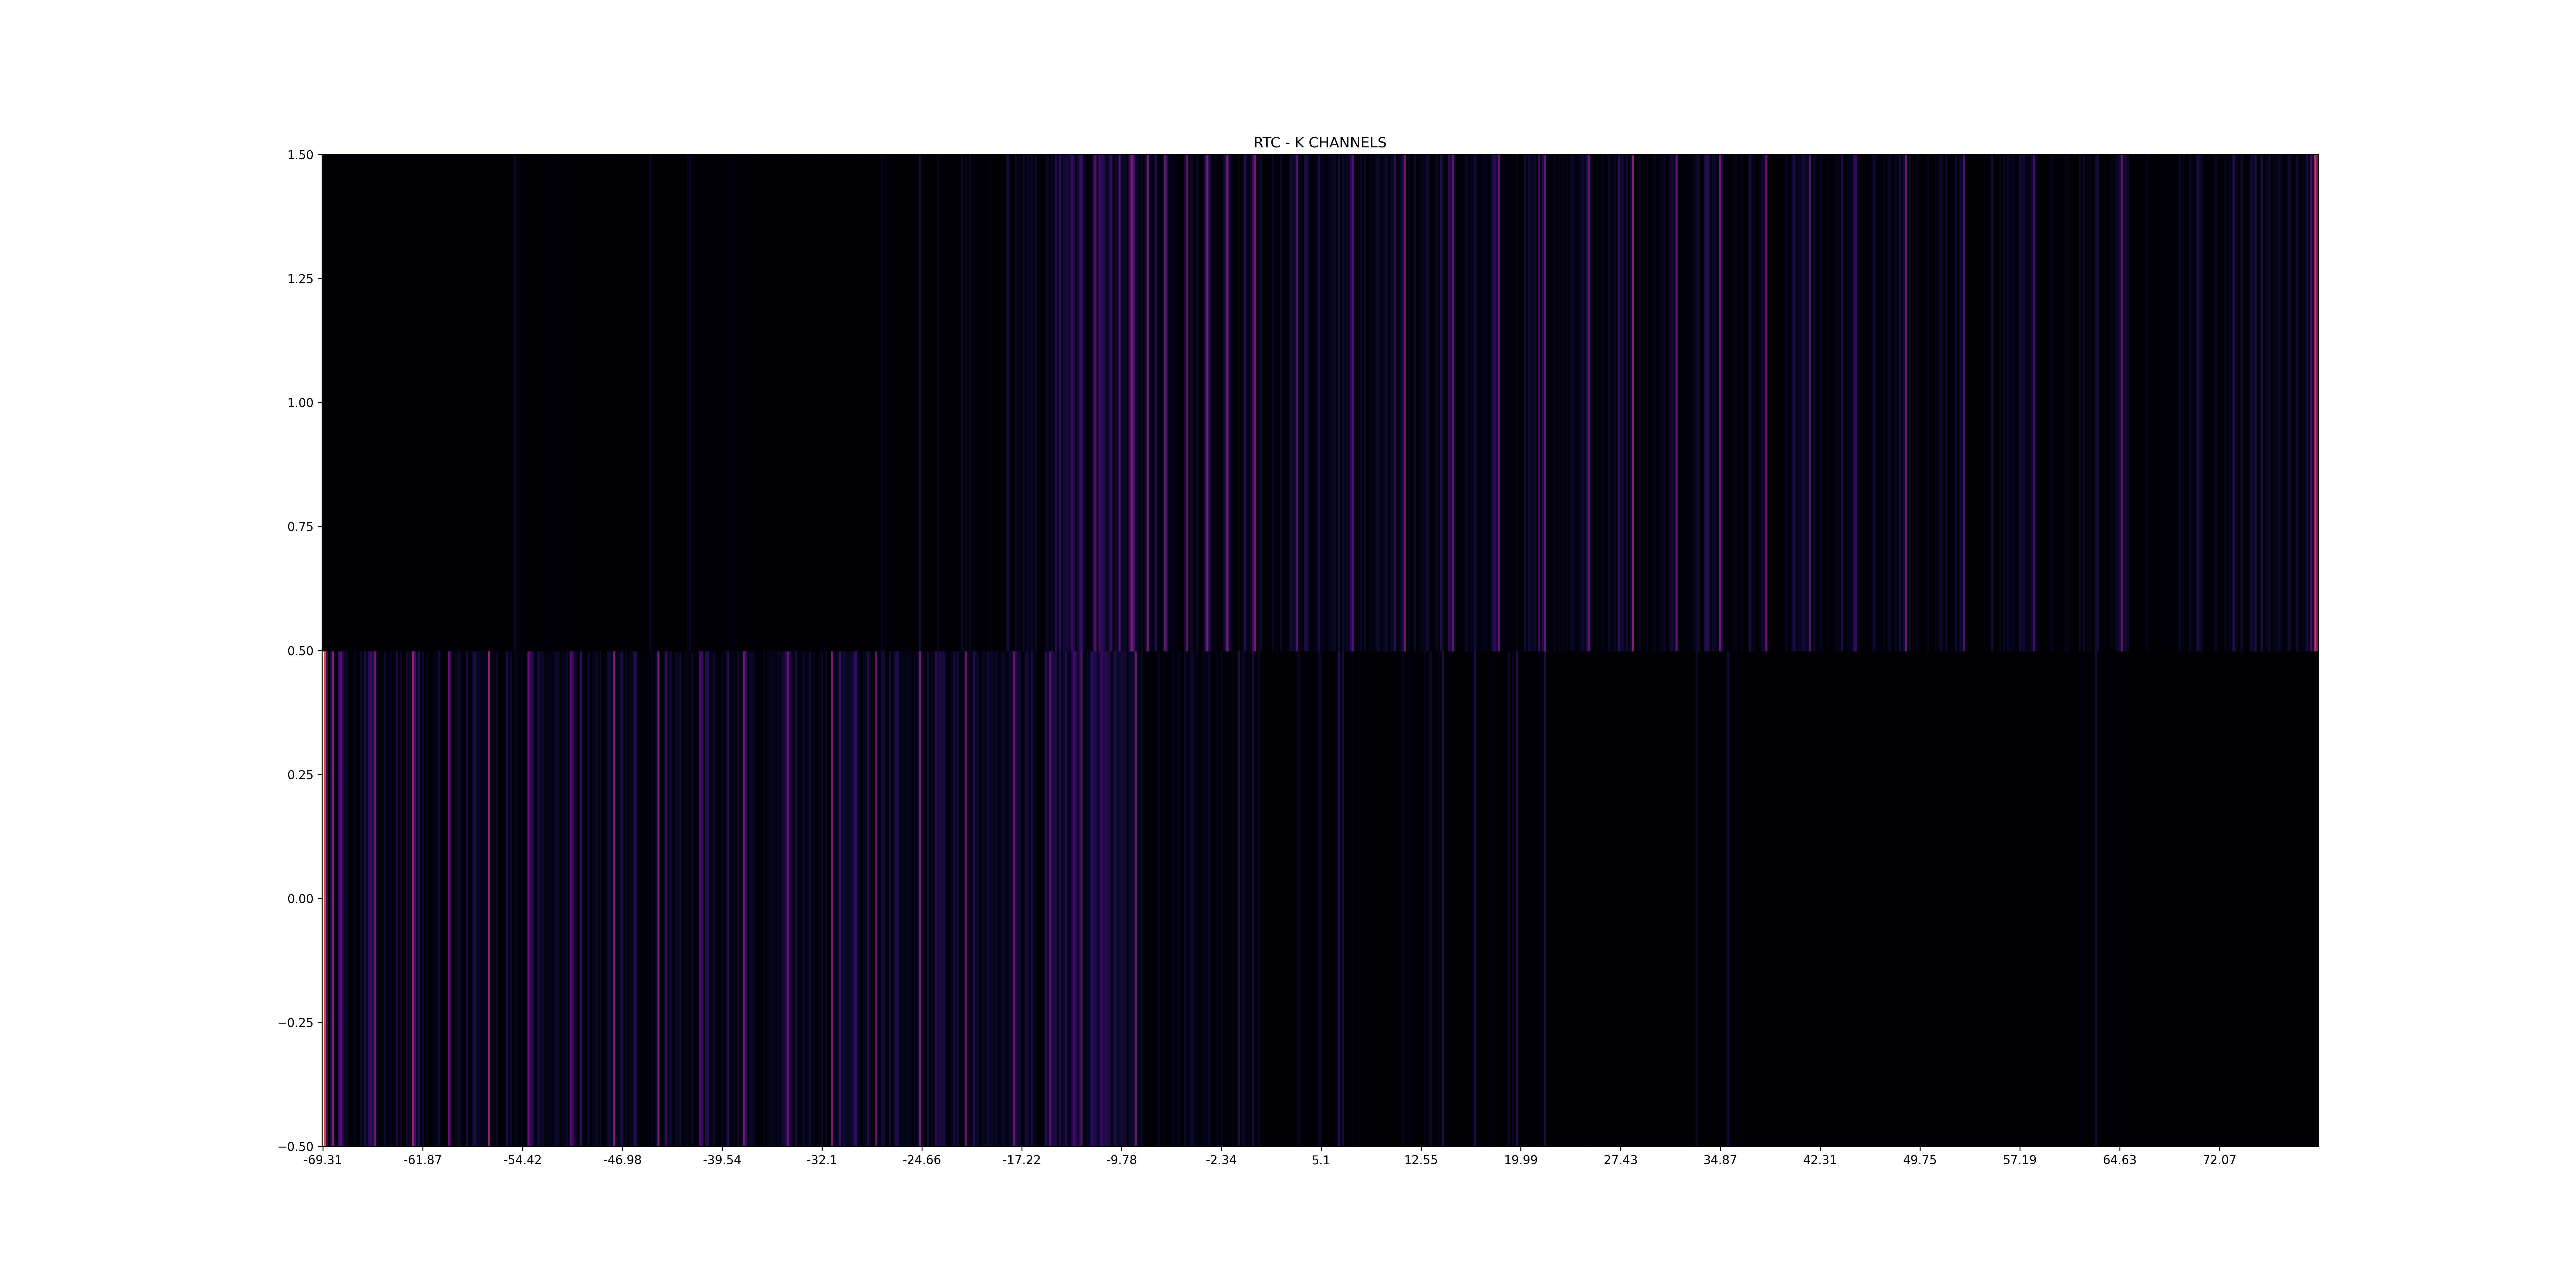
\includegraphics[width=.45\linewidth,valign=m]{Figures/1/K_RTC_.png} &
        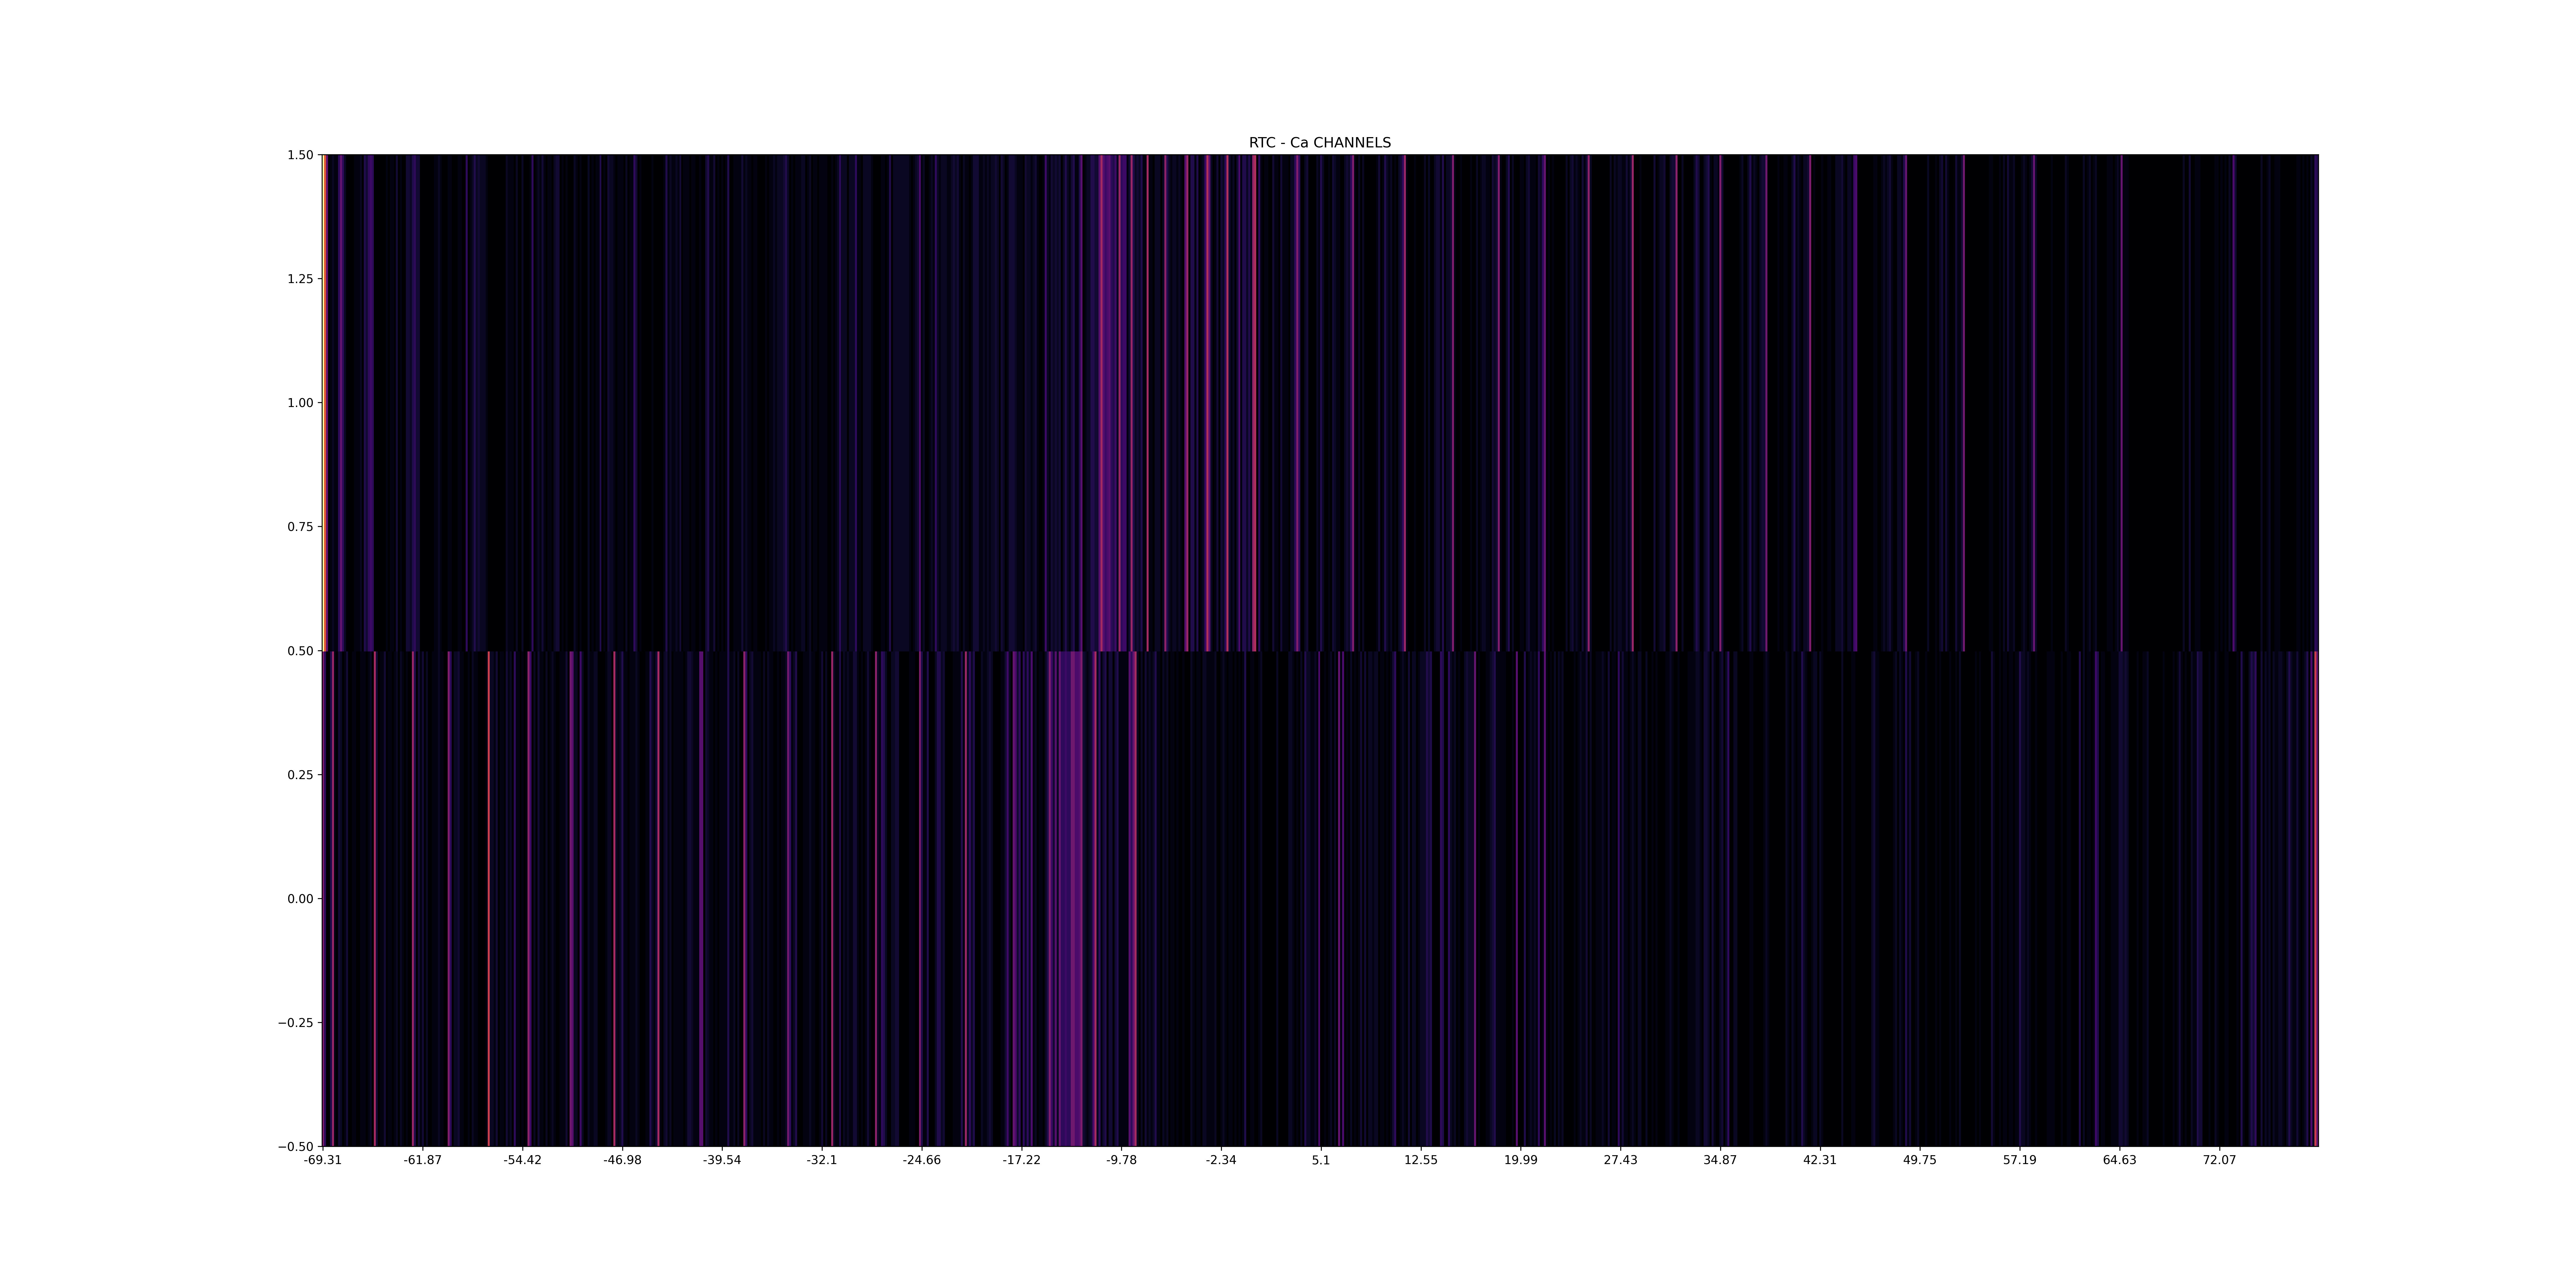
\includegraphics[width=.45\linewidth,valign=m]{Figures/1/Ca_RTC_.png} \\
        Gillespie &
        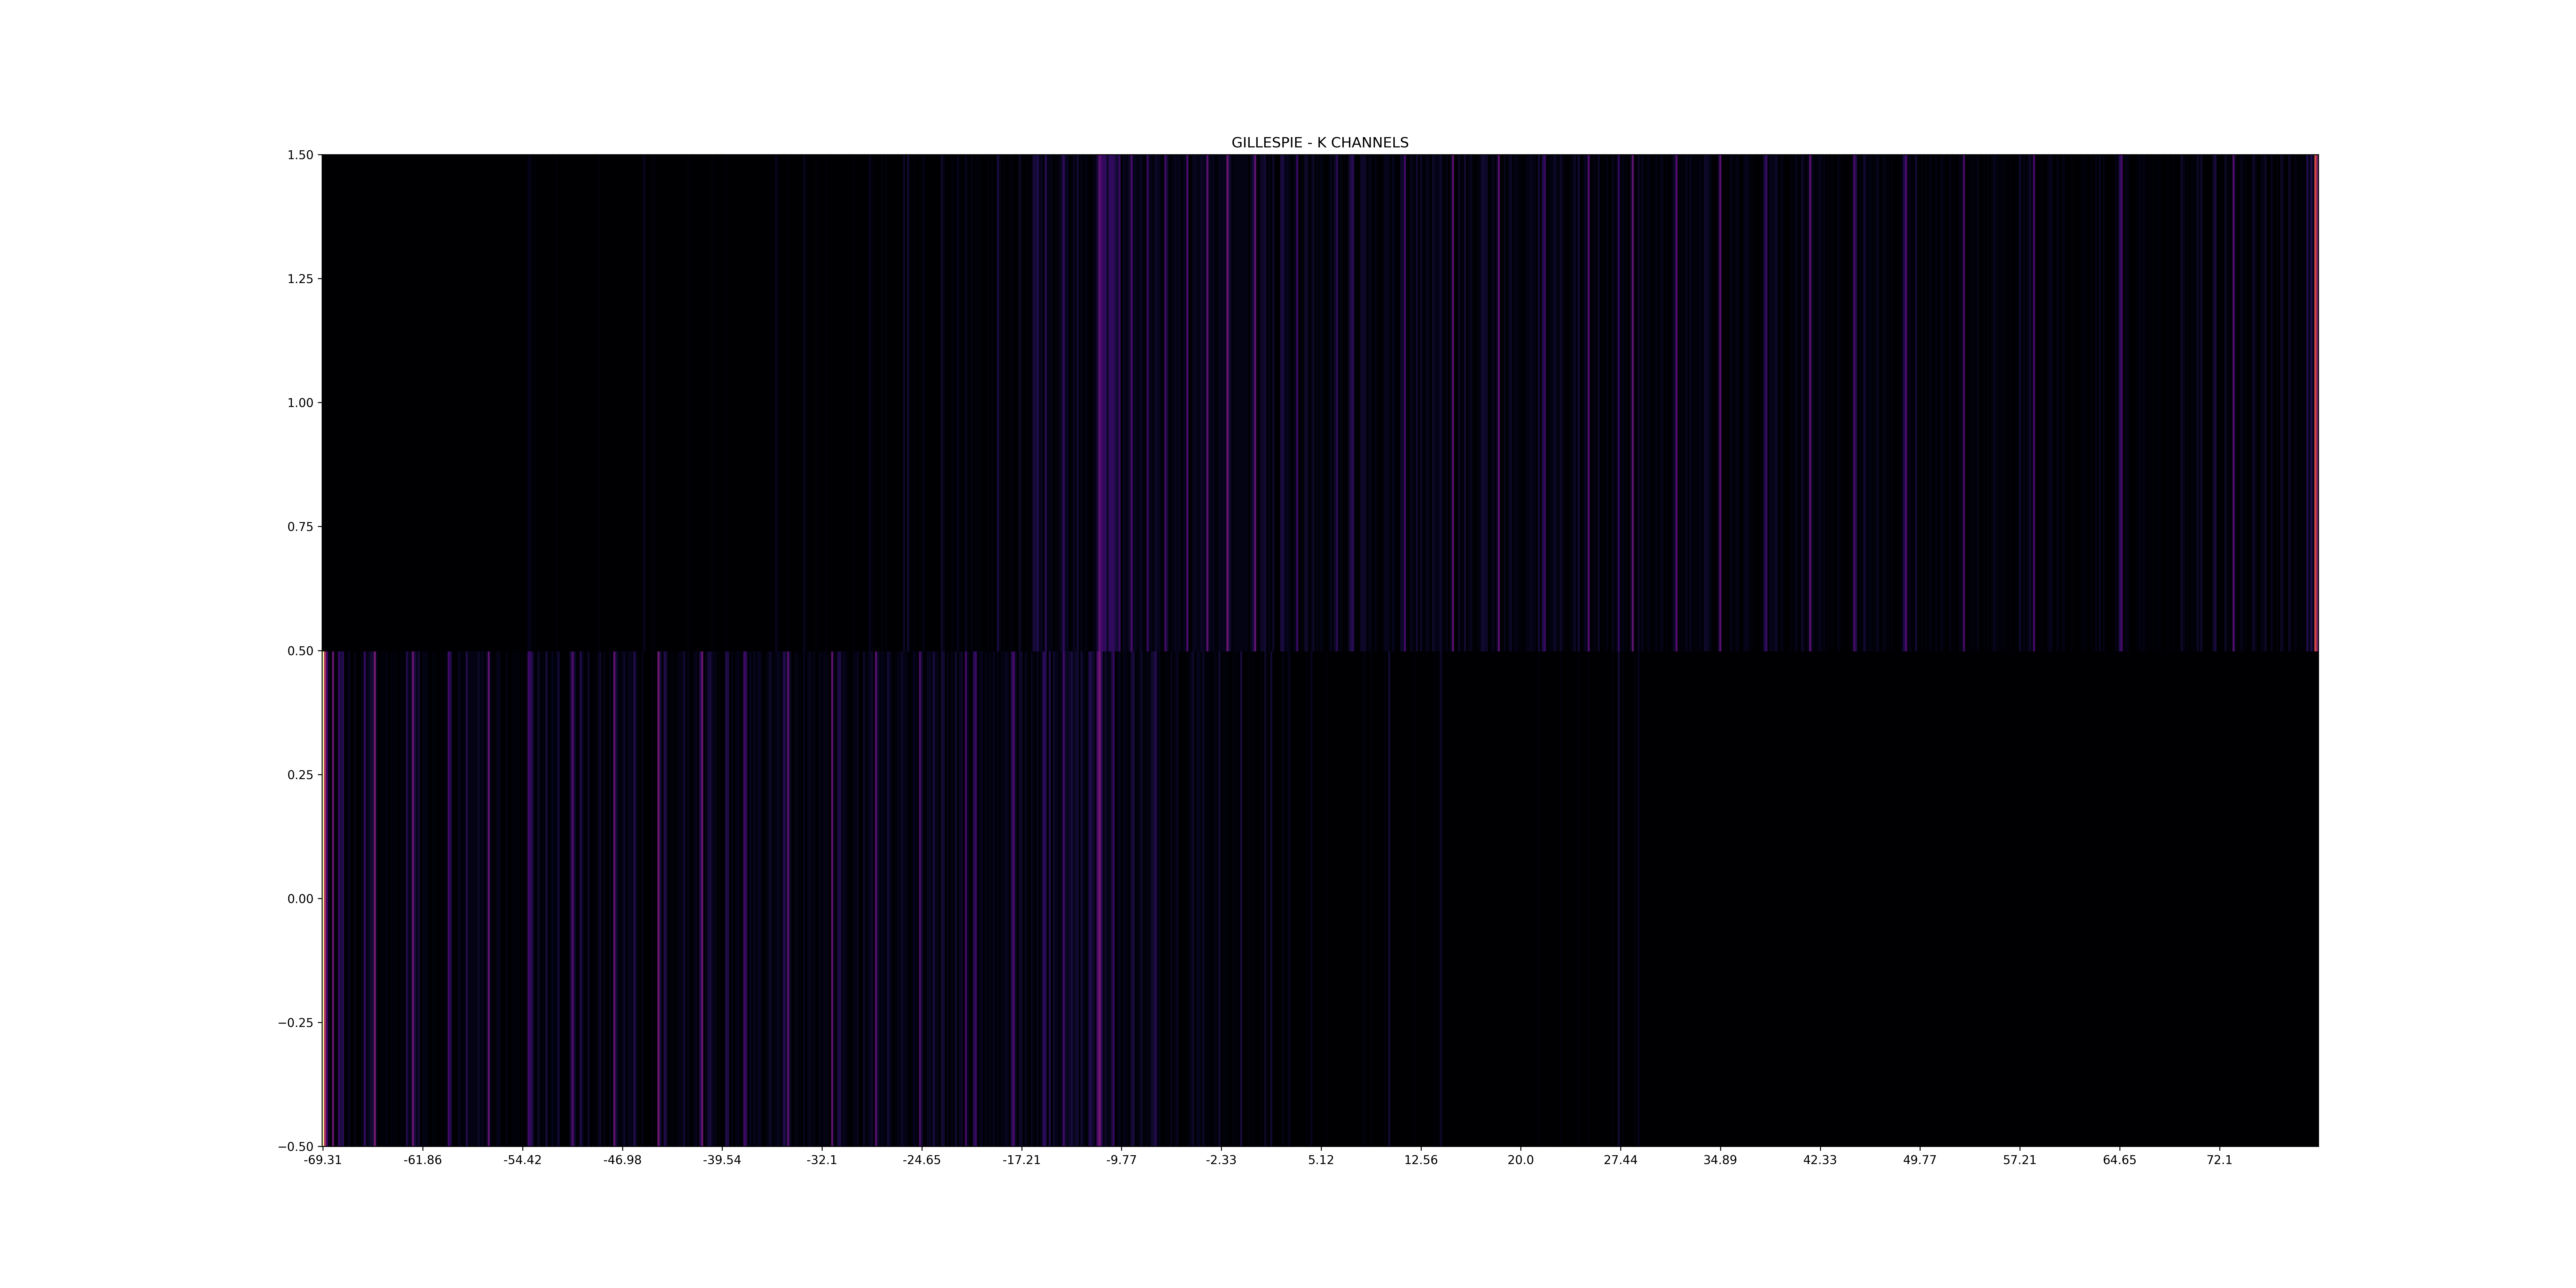
\includegraphics[width=.45\linewidth,valign=m]{Figures/1/K_GILLESPIE_.png} &
        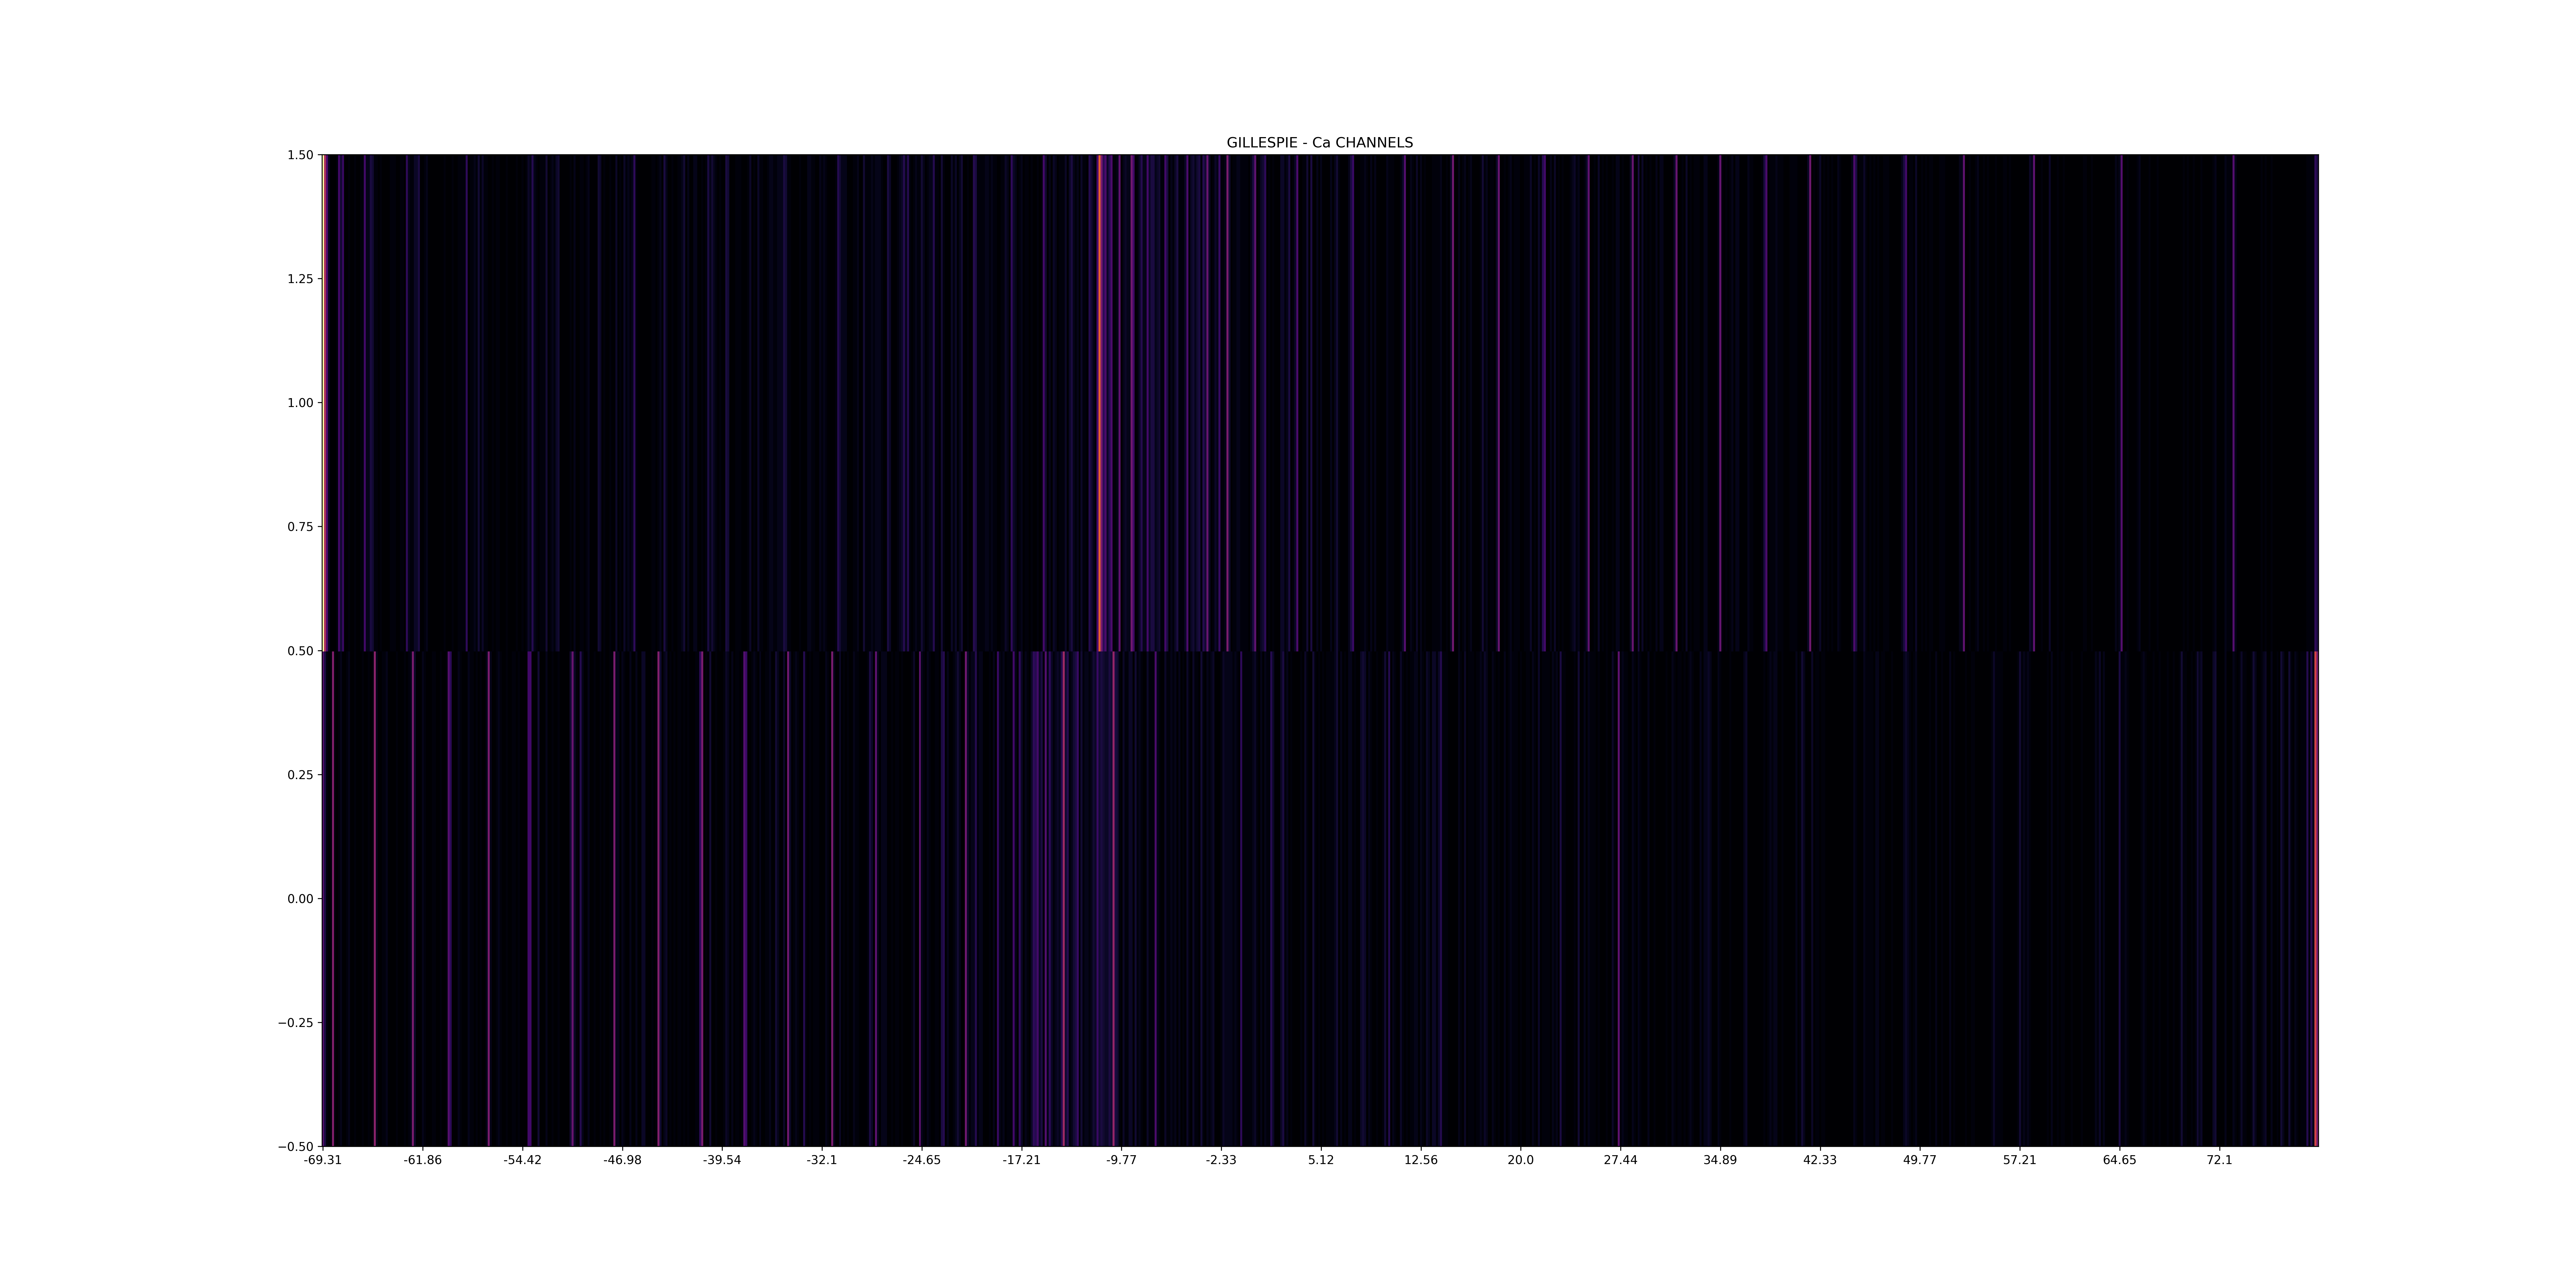
\includegraphics[width=.45\linewidth,valign=m]{Figures/1/Ca_GILLESPIE_.png} \\
        \end{tabular}
    \caption{Heatmap of the RTC and Gillespie representations using one channel for each type}
    \label{tab:my_label}
\end{table}

\begin{table}[]
    \centering
    \begin{tabular}{ccc}
        & Potassium & Calcium\\
        RTC &
        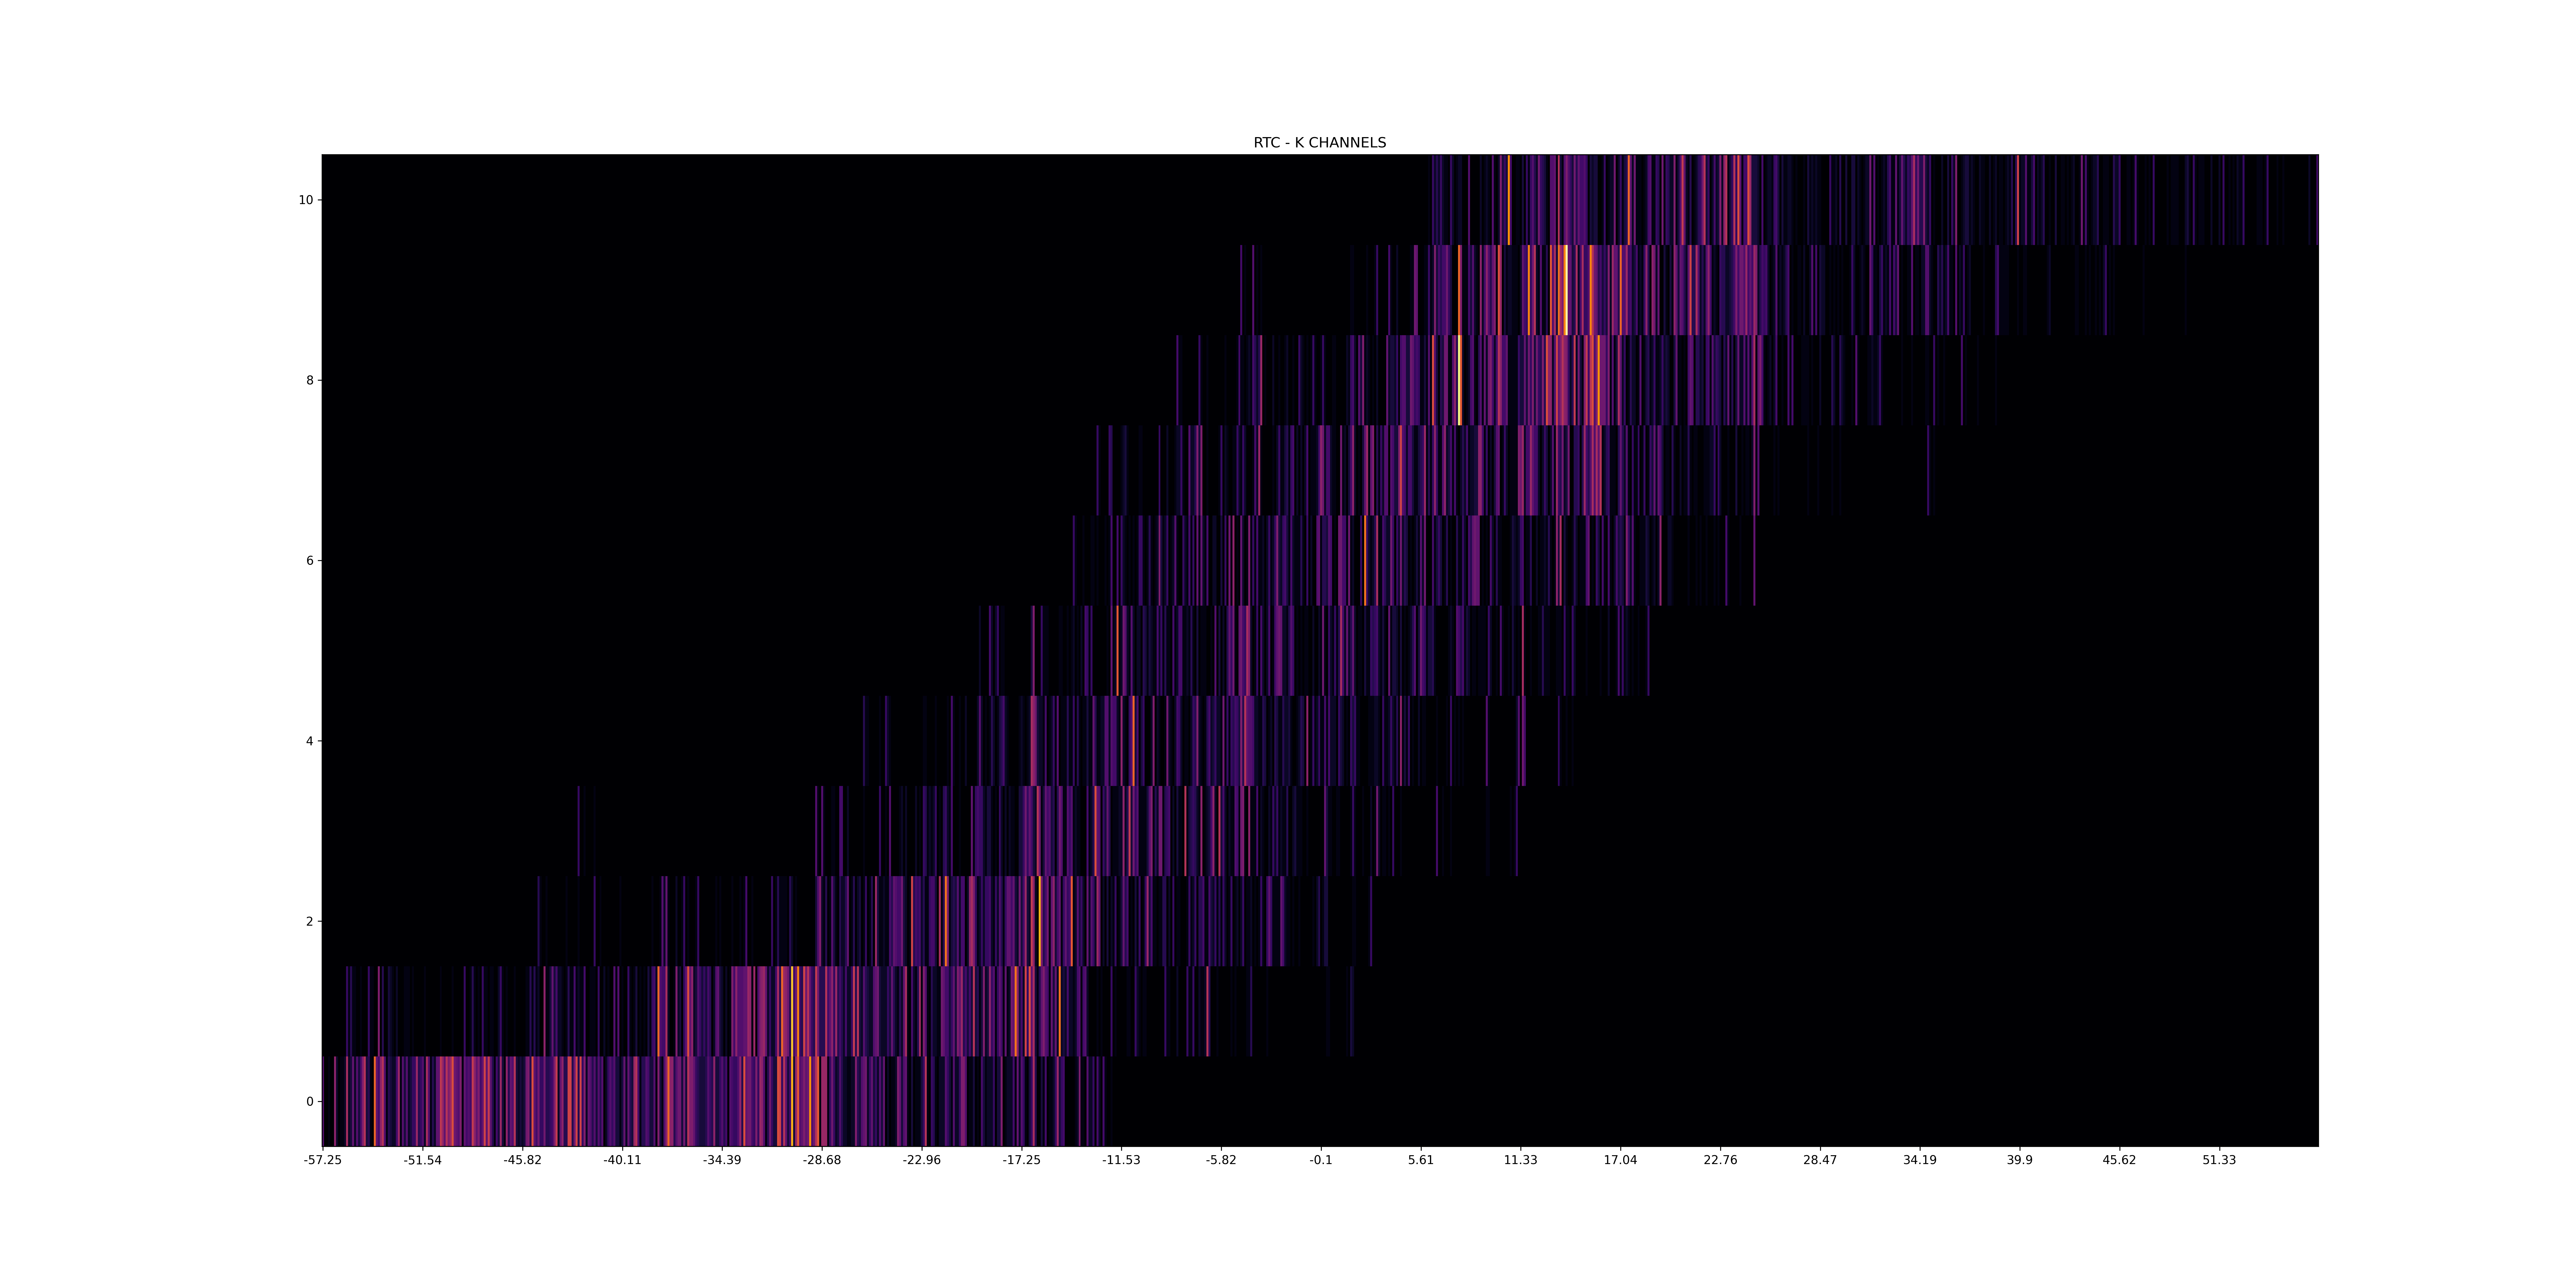
\includegraphics[width=.45\linewidth,valign=m]{Figures/10/K_RTC_.png} &
        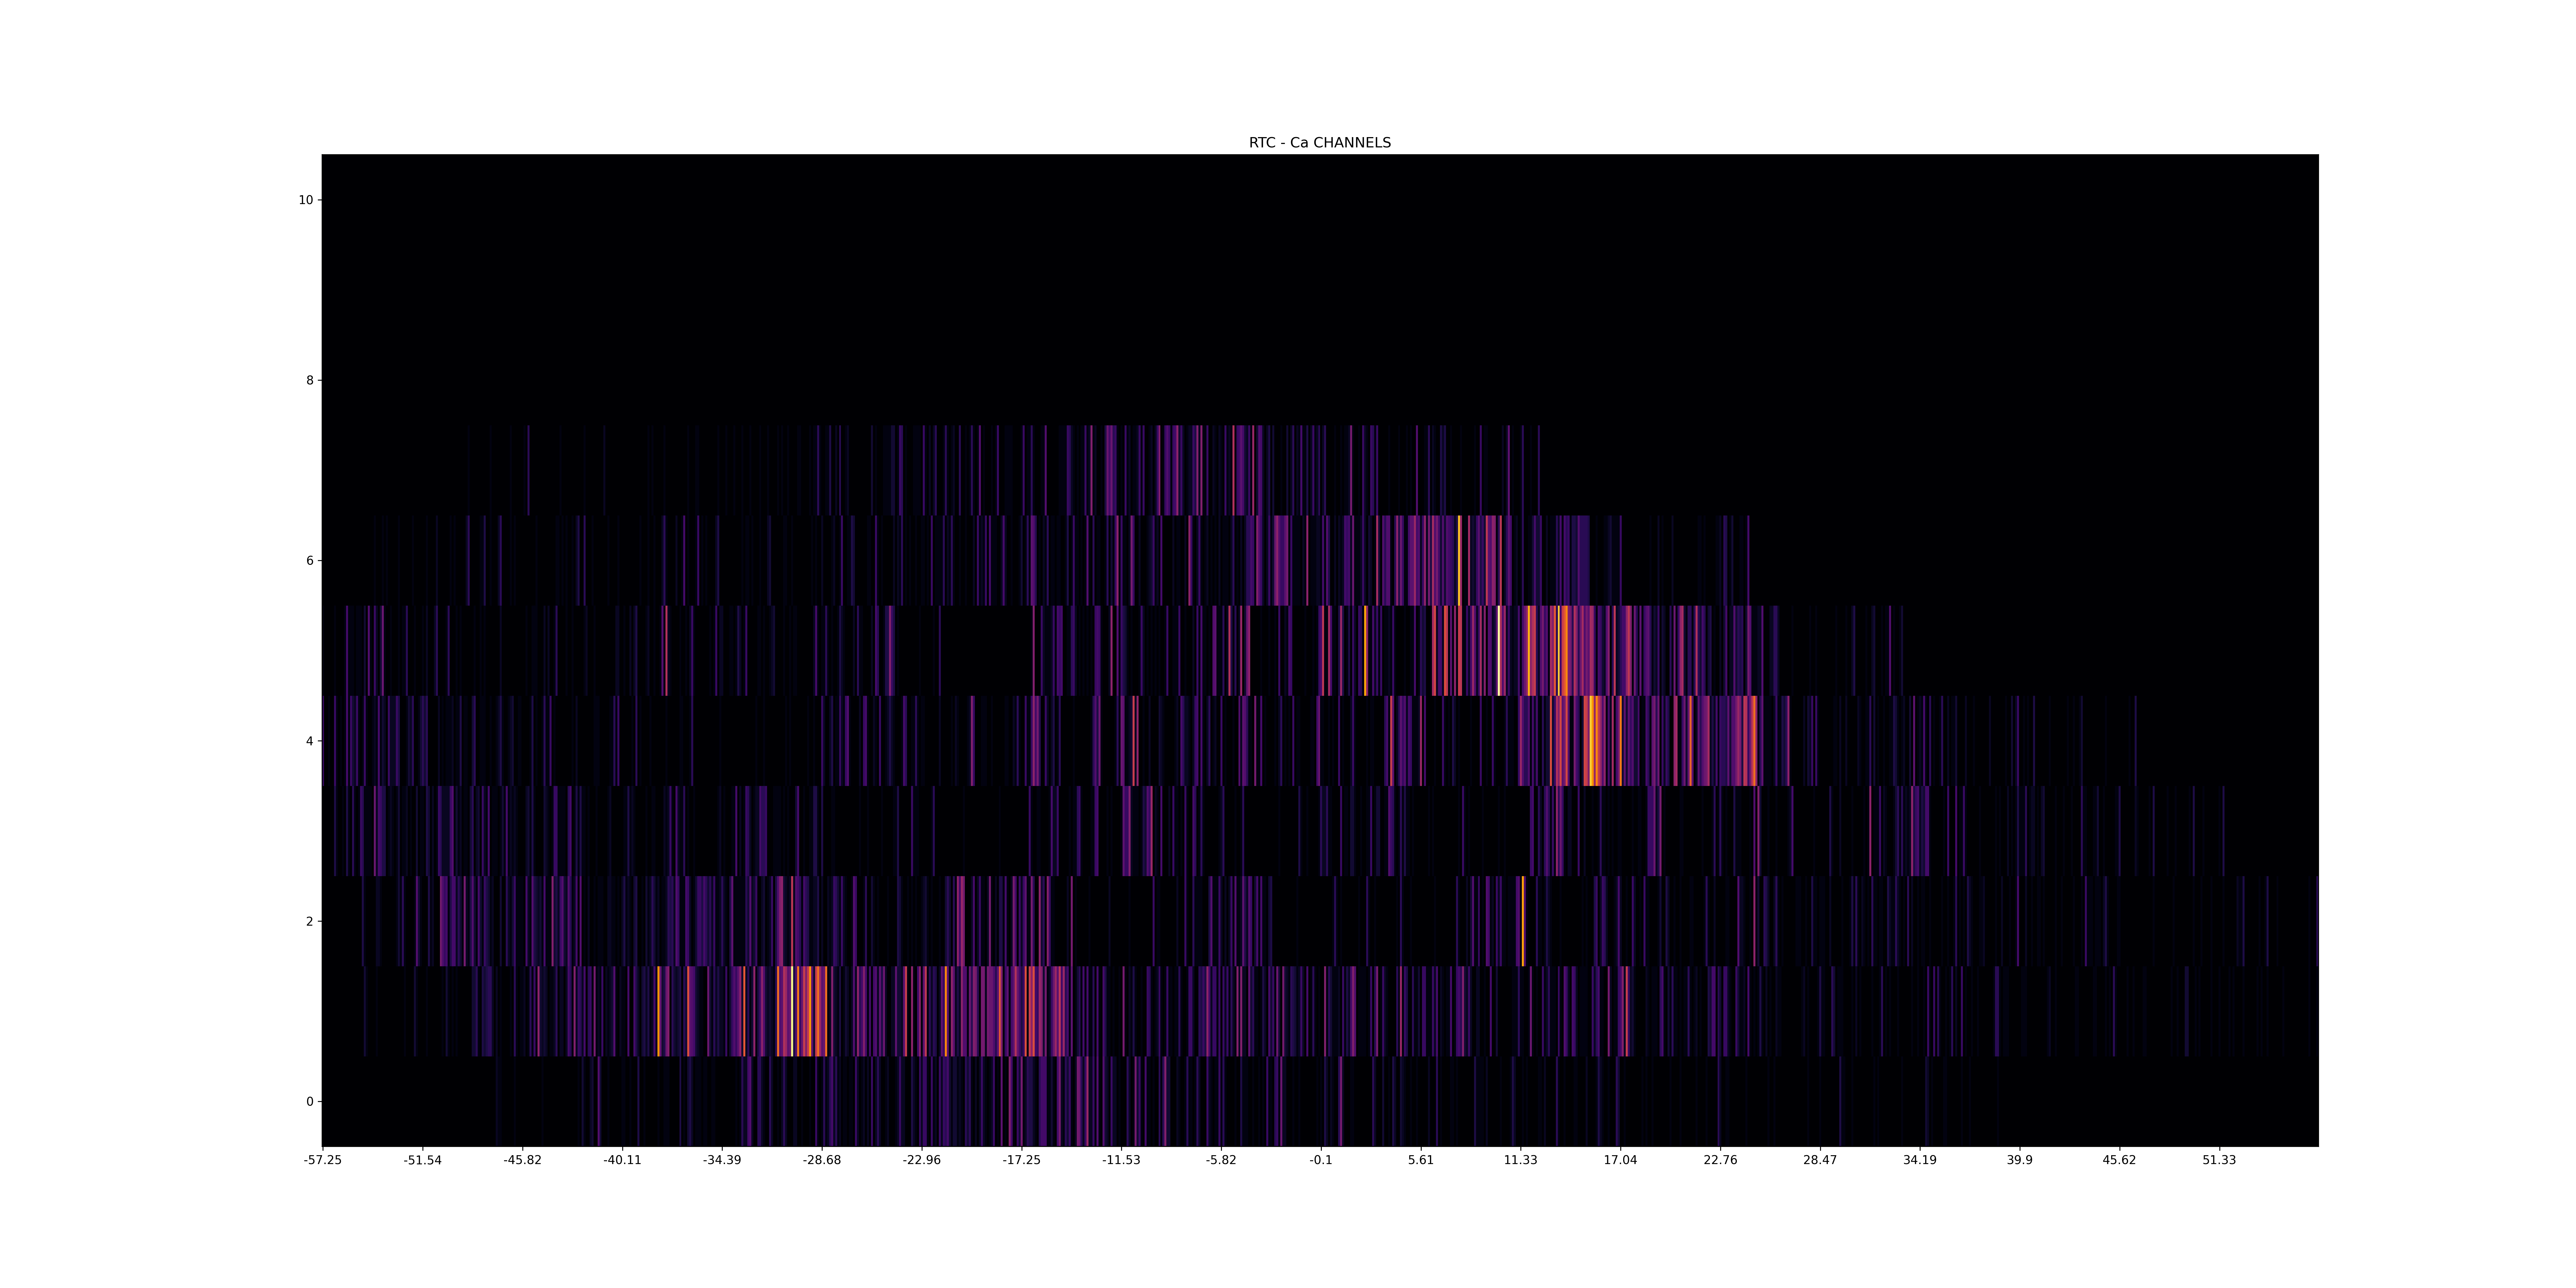
\includegraphics[width=.45\linewidth,valign=m]{Figures/10/Ca_RTC_.png} \\
        Gillespie &
        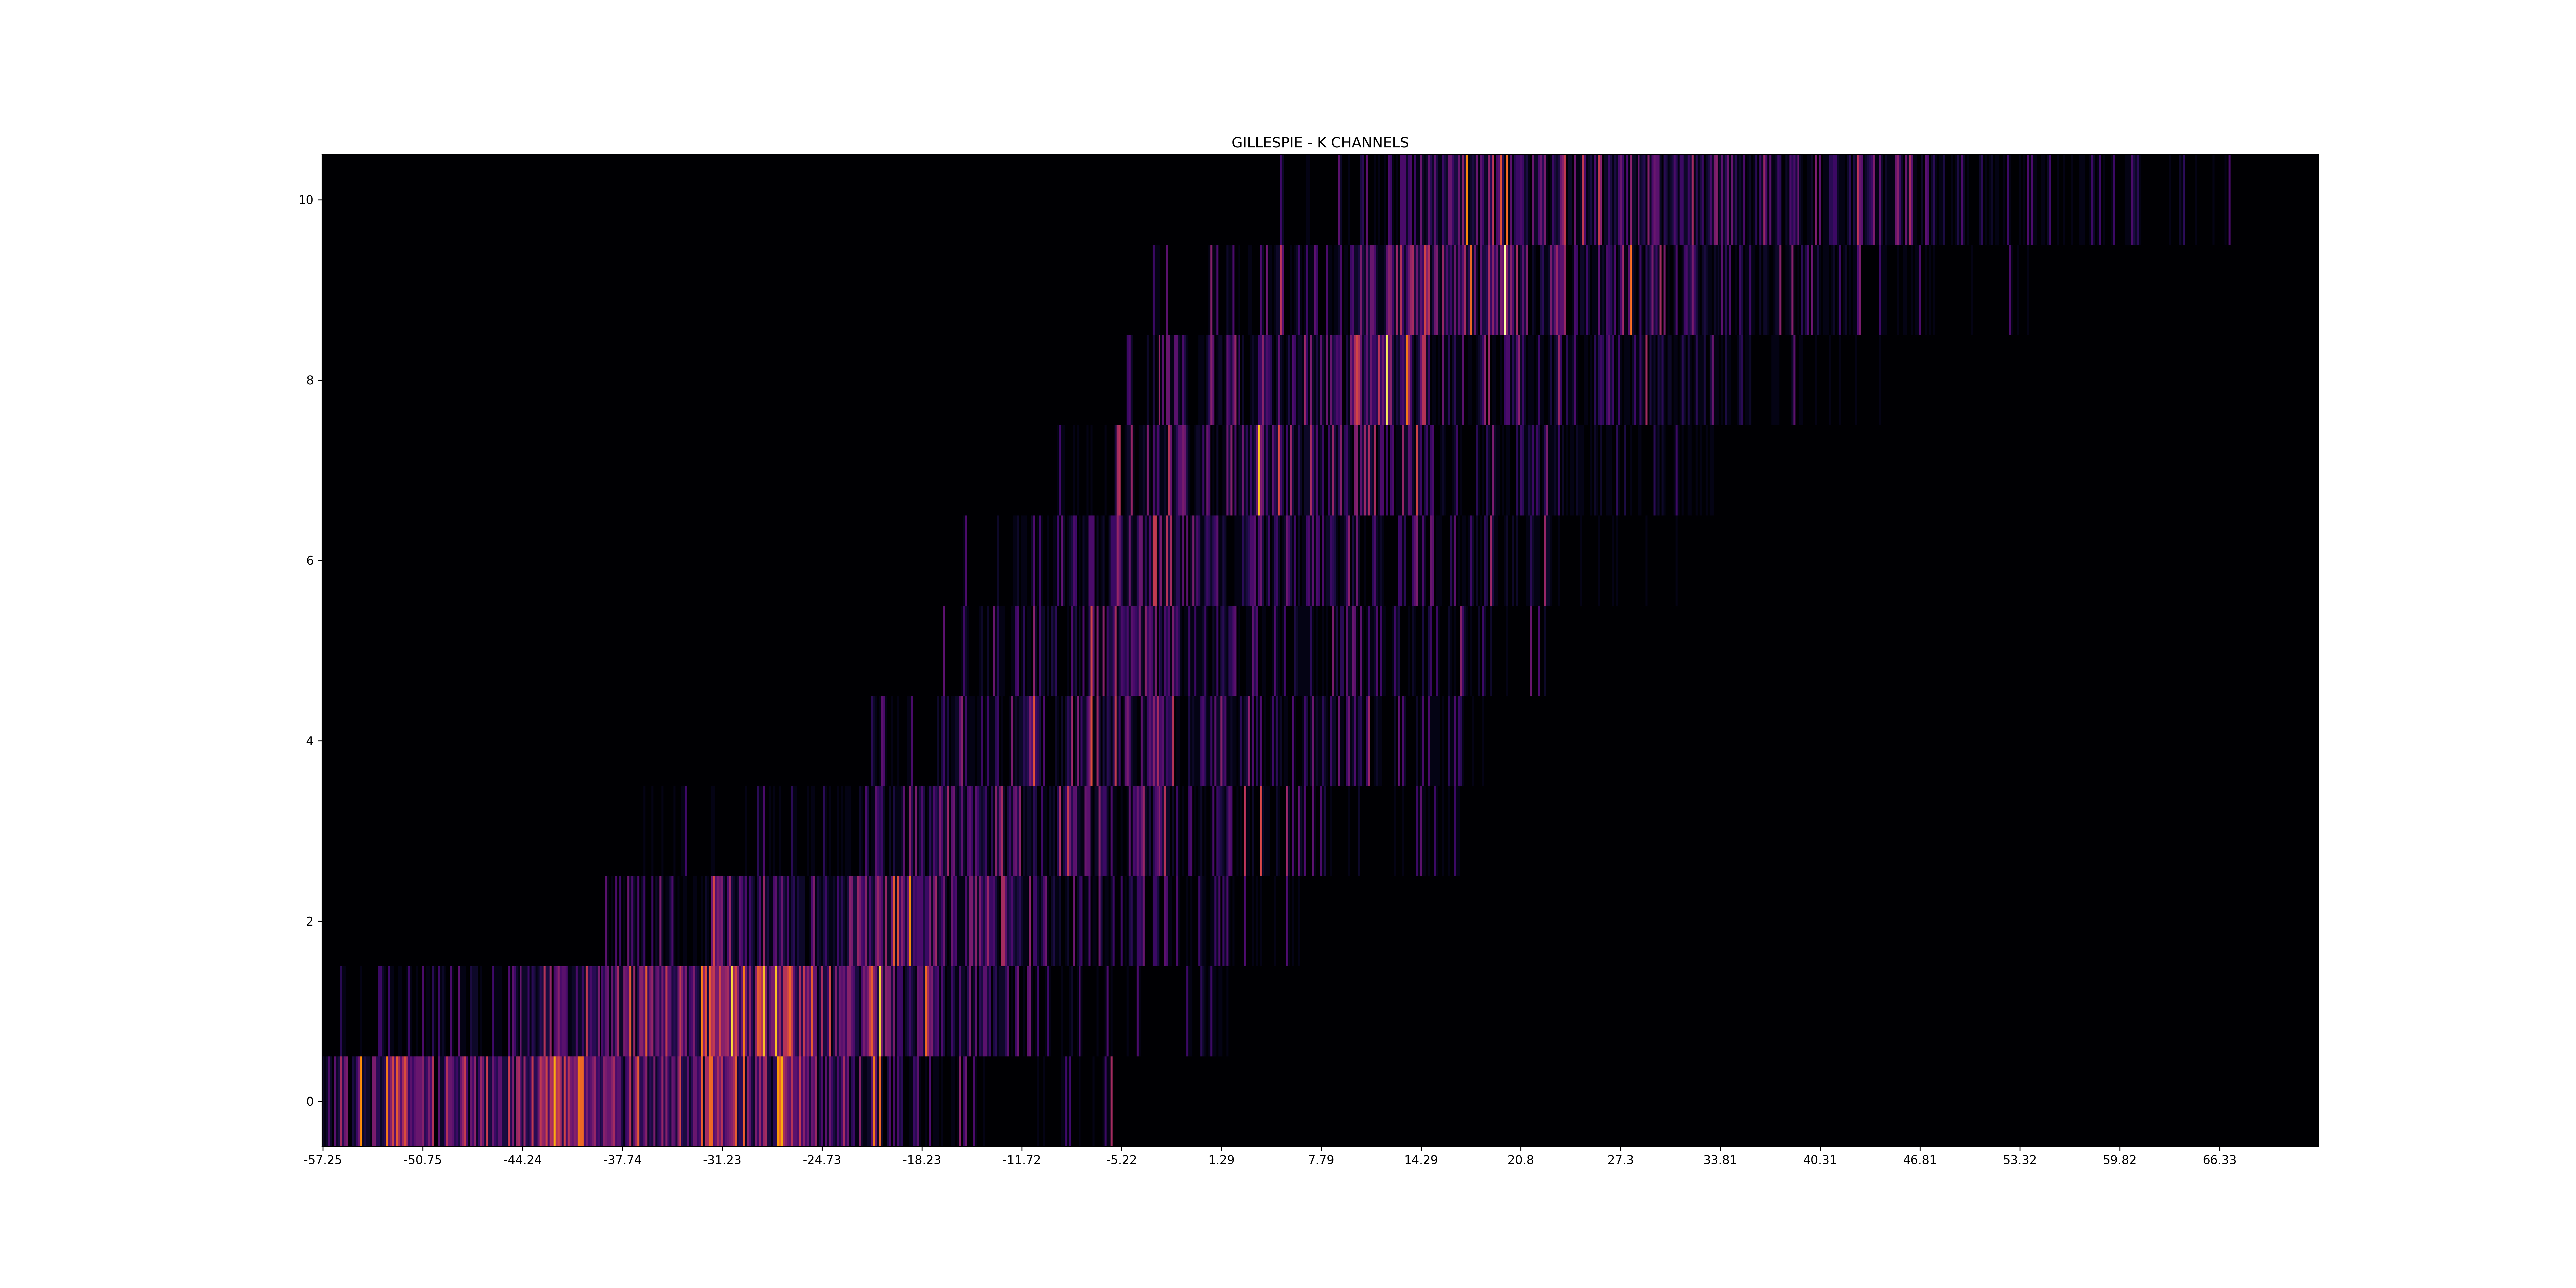
\includegraphics[width=.45\linewidth,valign=m]{Figures/10/K_GILLESPIE_.png} &
        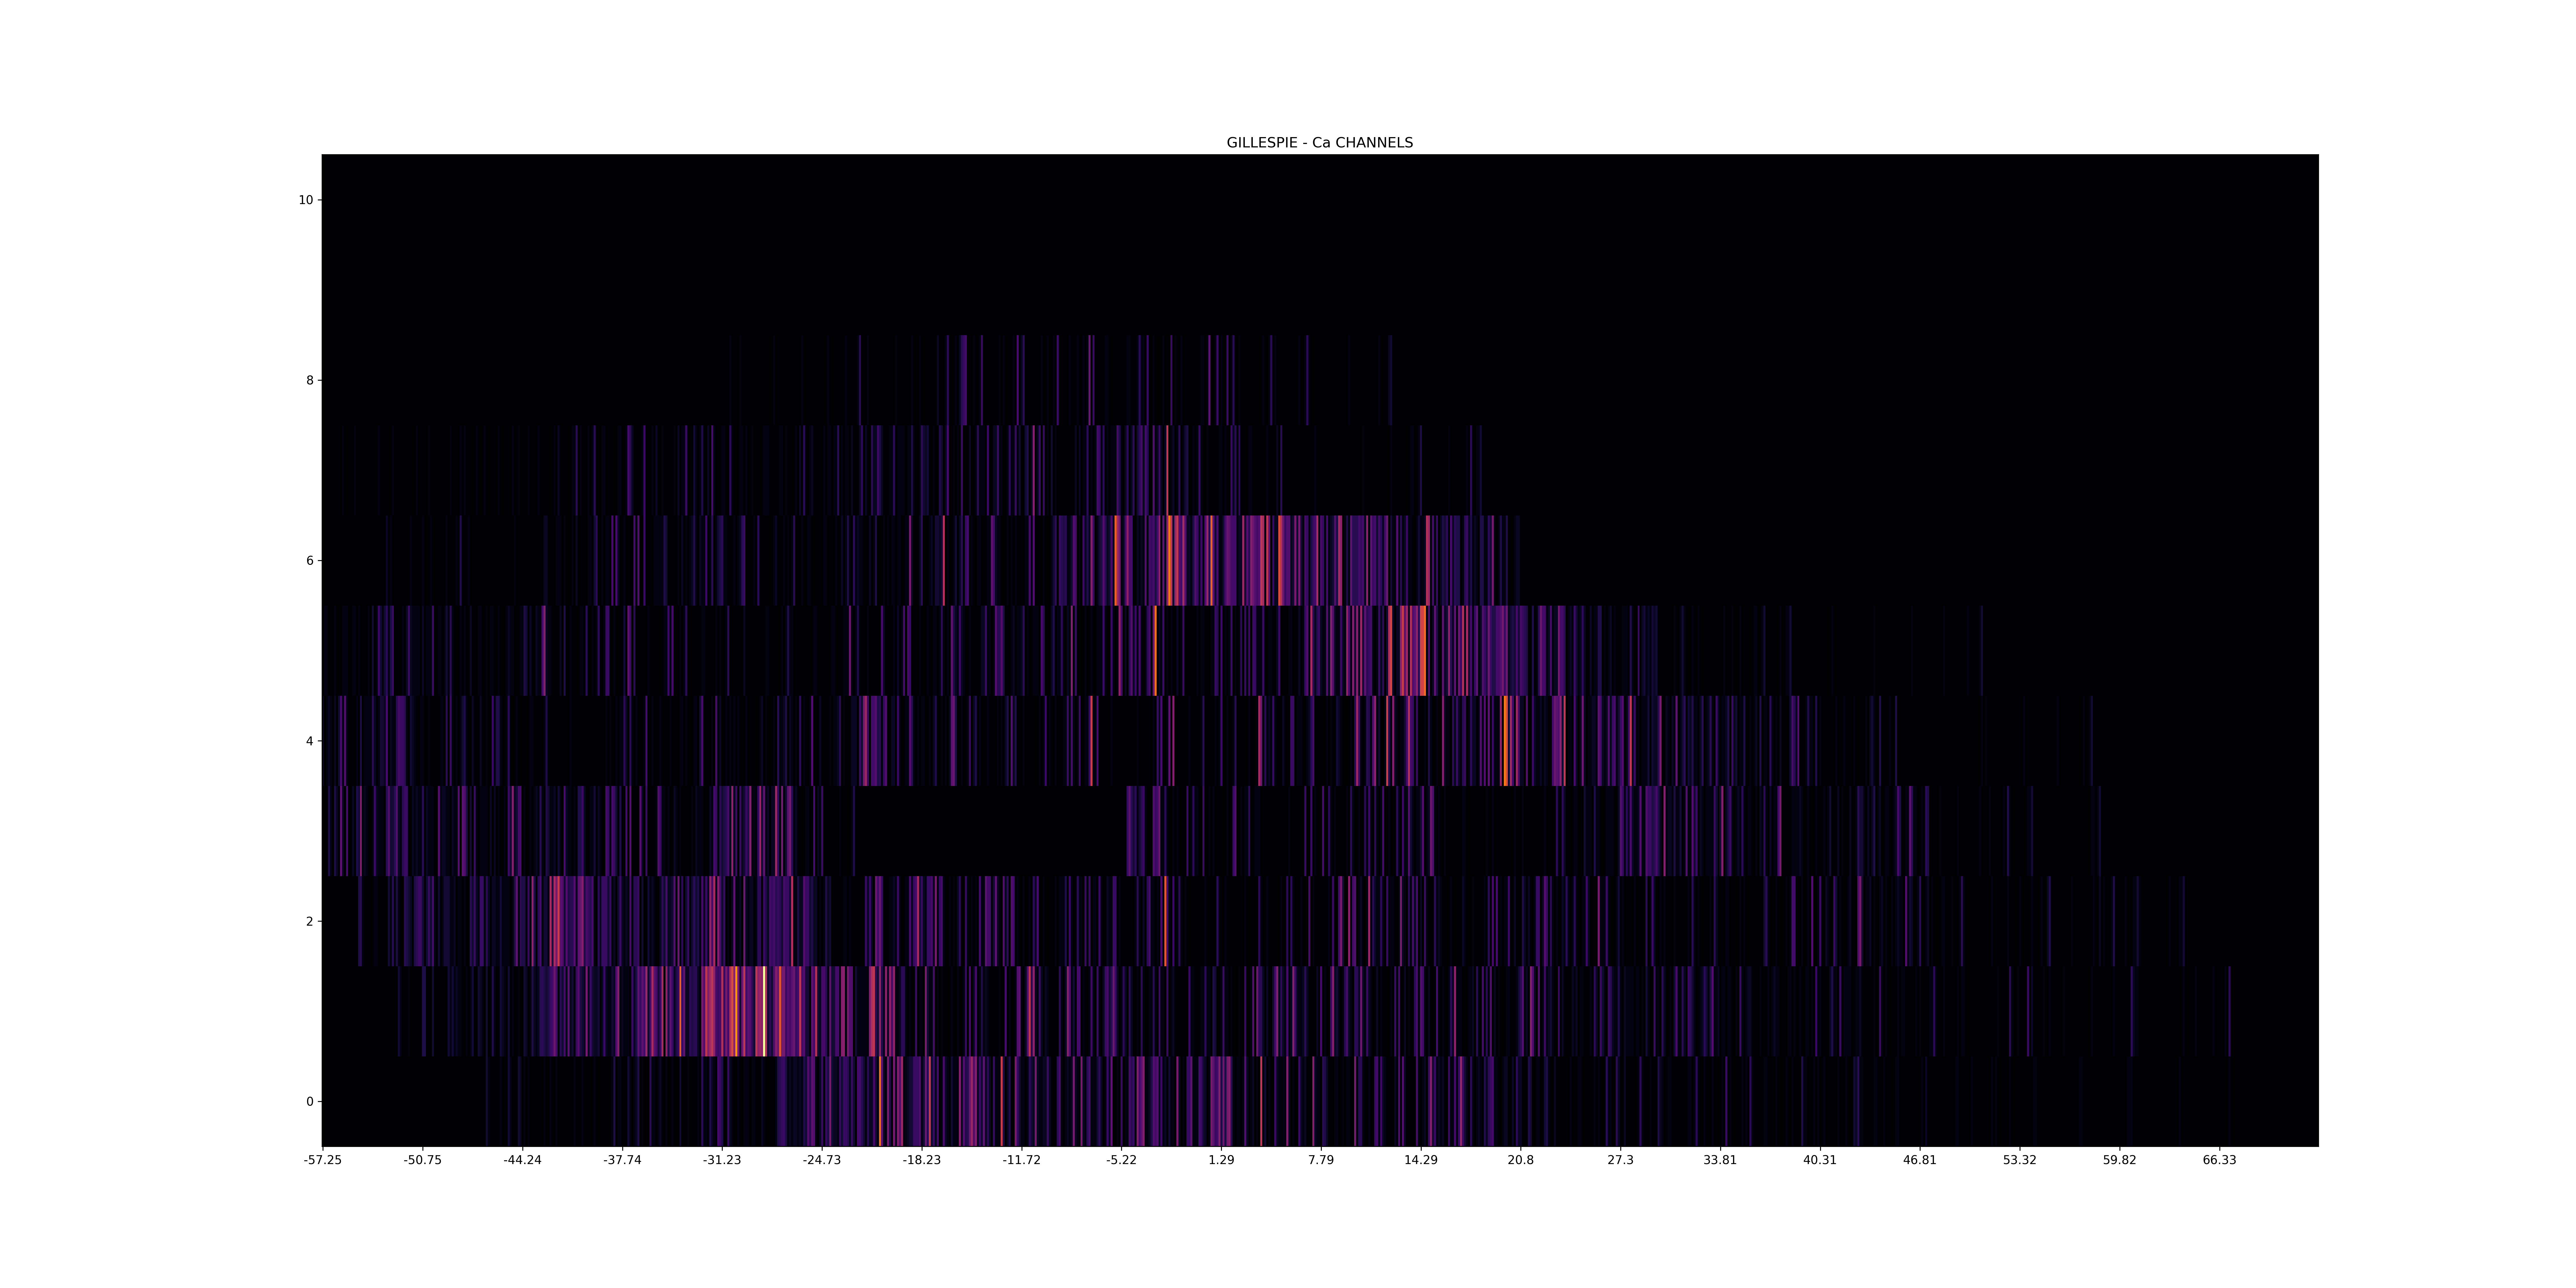
\includegraphics[width=.45\linewidth,valign=m]{Figures/10/Ca_GILLESPIE_.png} \\
    \end{tabular}
    \caption{Heatmap of the RTC and Gillespie representations using ten channels for each type}
    \label{tab:my_label}
\end{table}


\begin{table}[]
    \centering
    \begin{tabular}{ccc}
    & Potassium & Calcium\\
    RTC &
    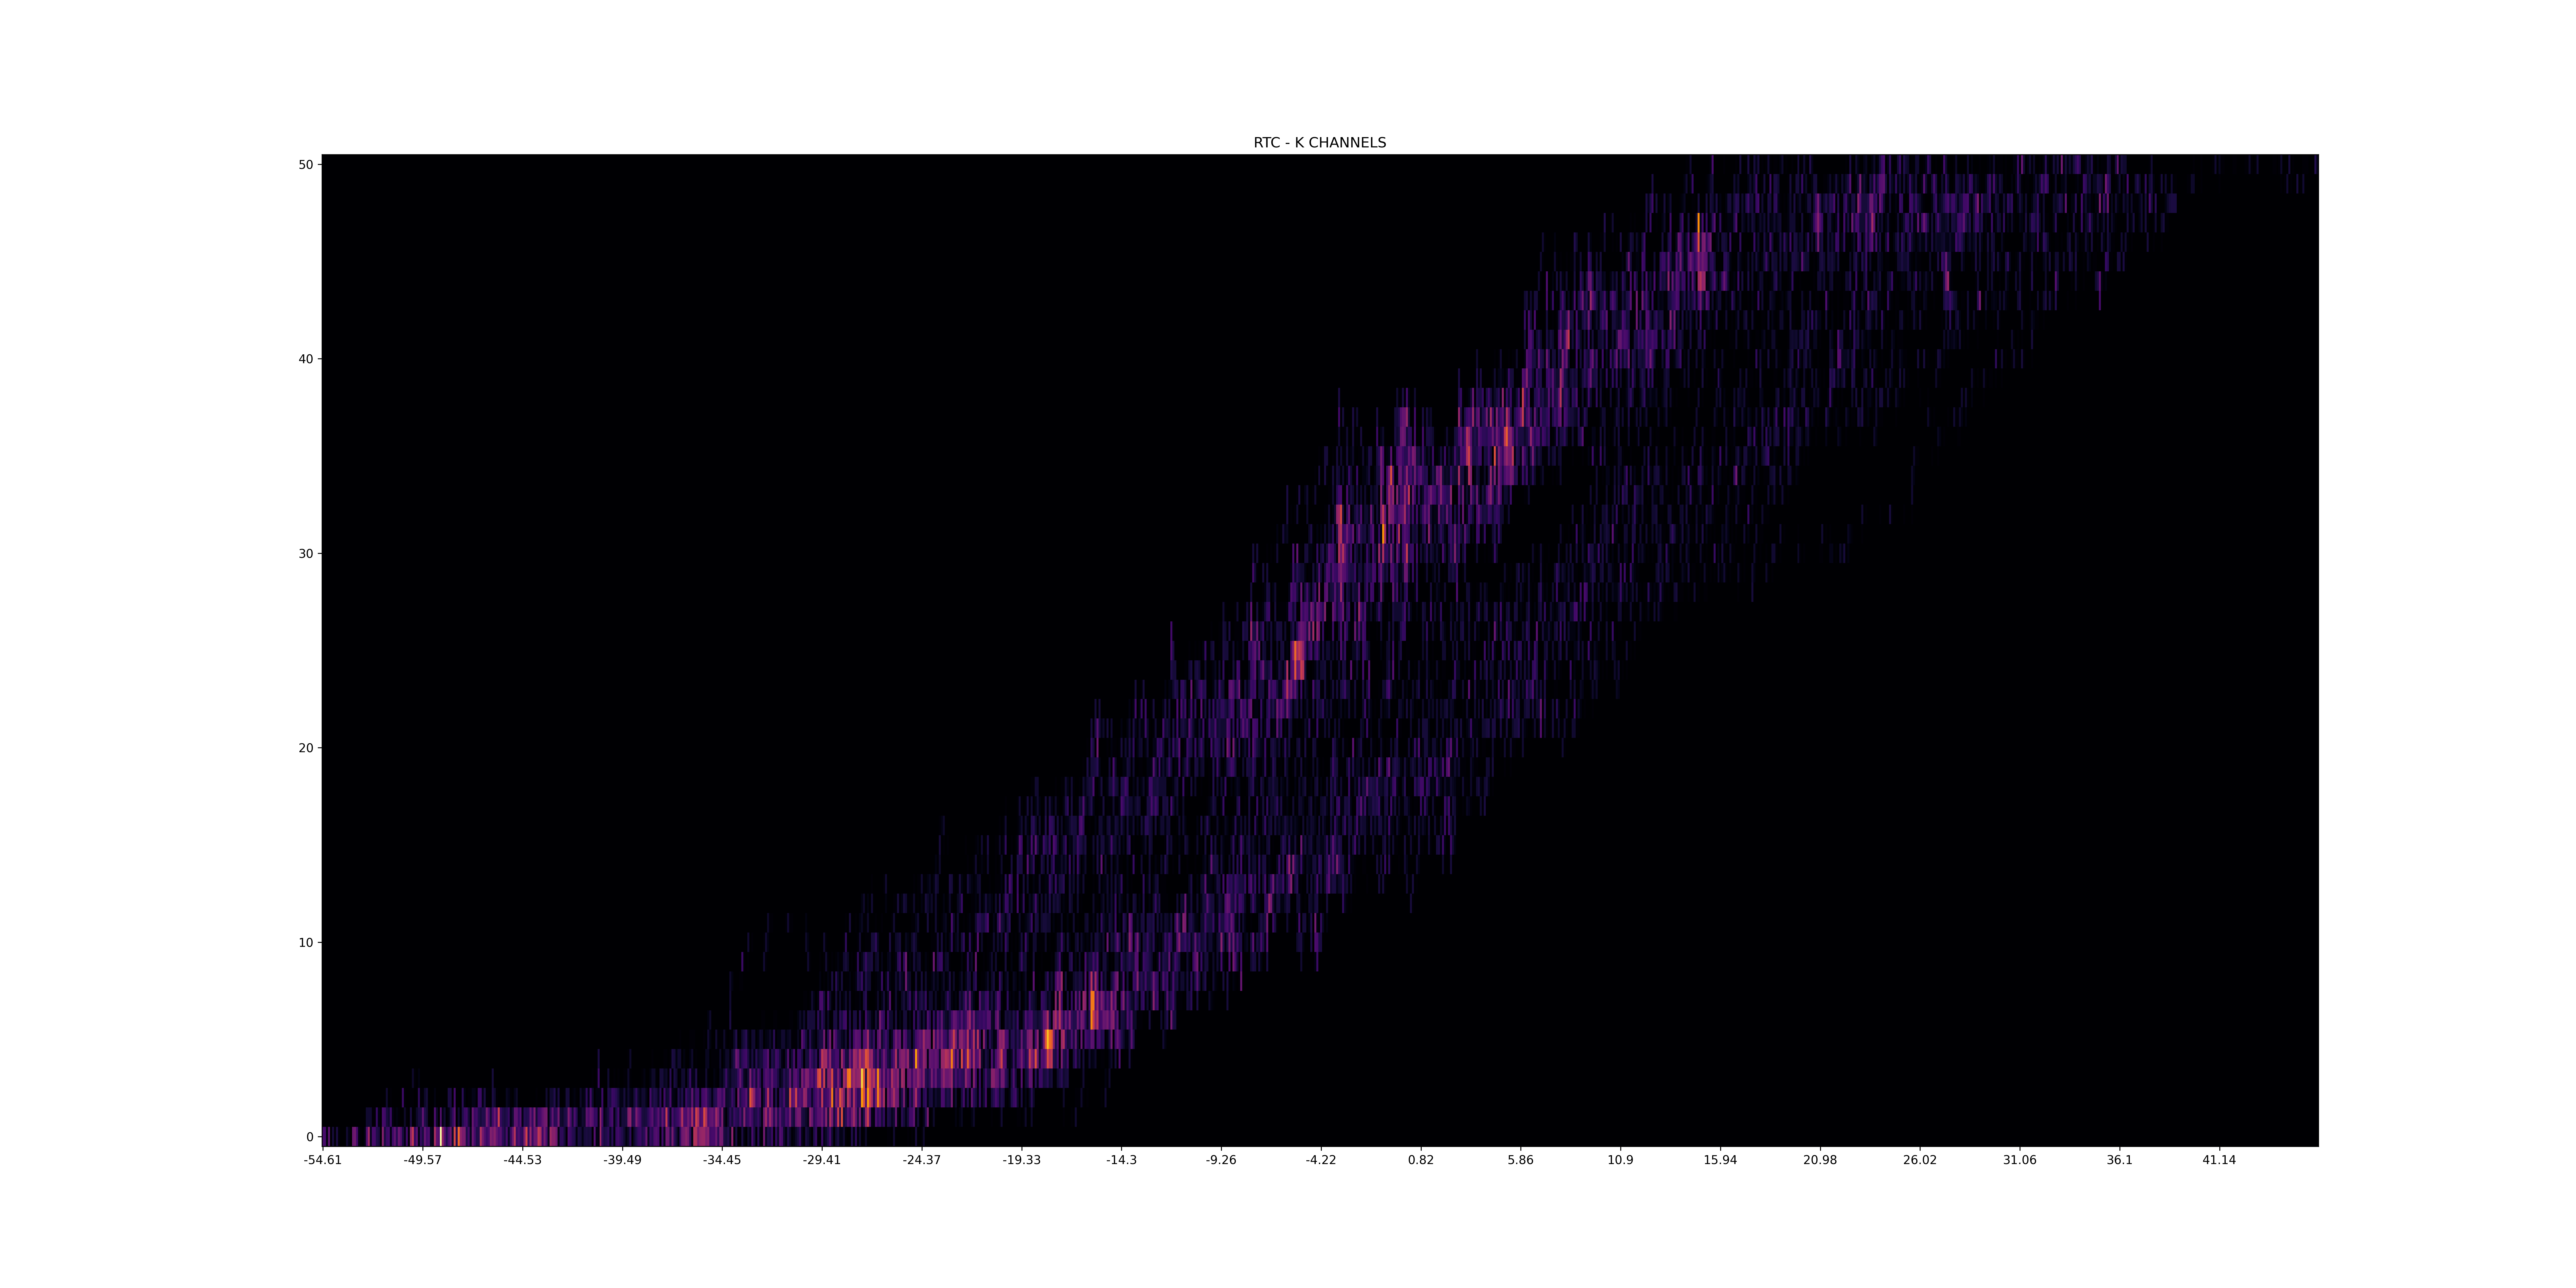
\includegraphics[width=.45\linewidth,valign=m]{Figures/50/K_RTC_.png} &
    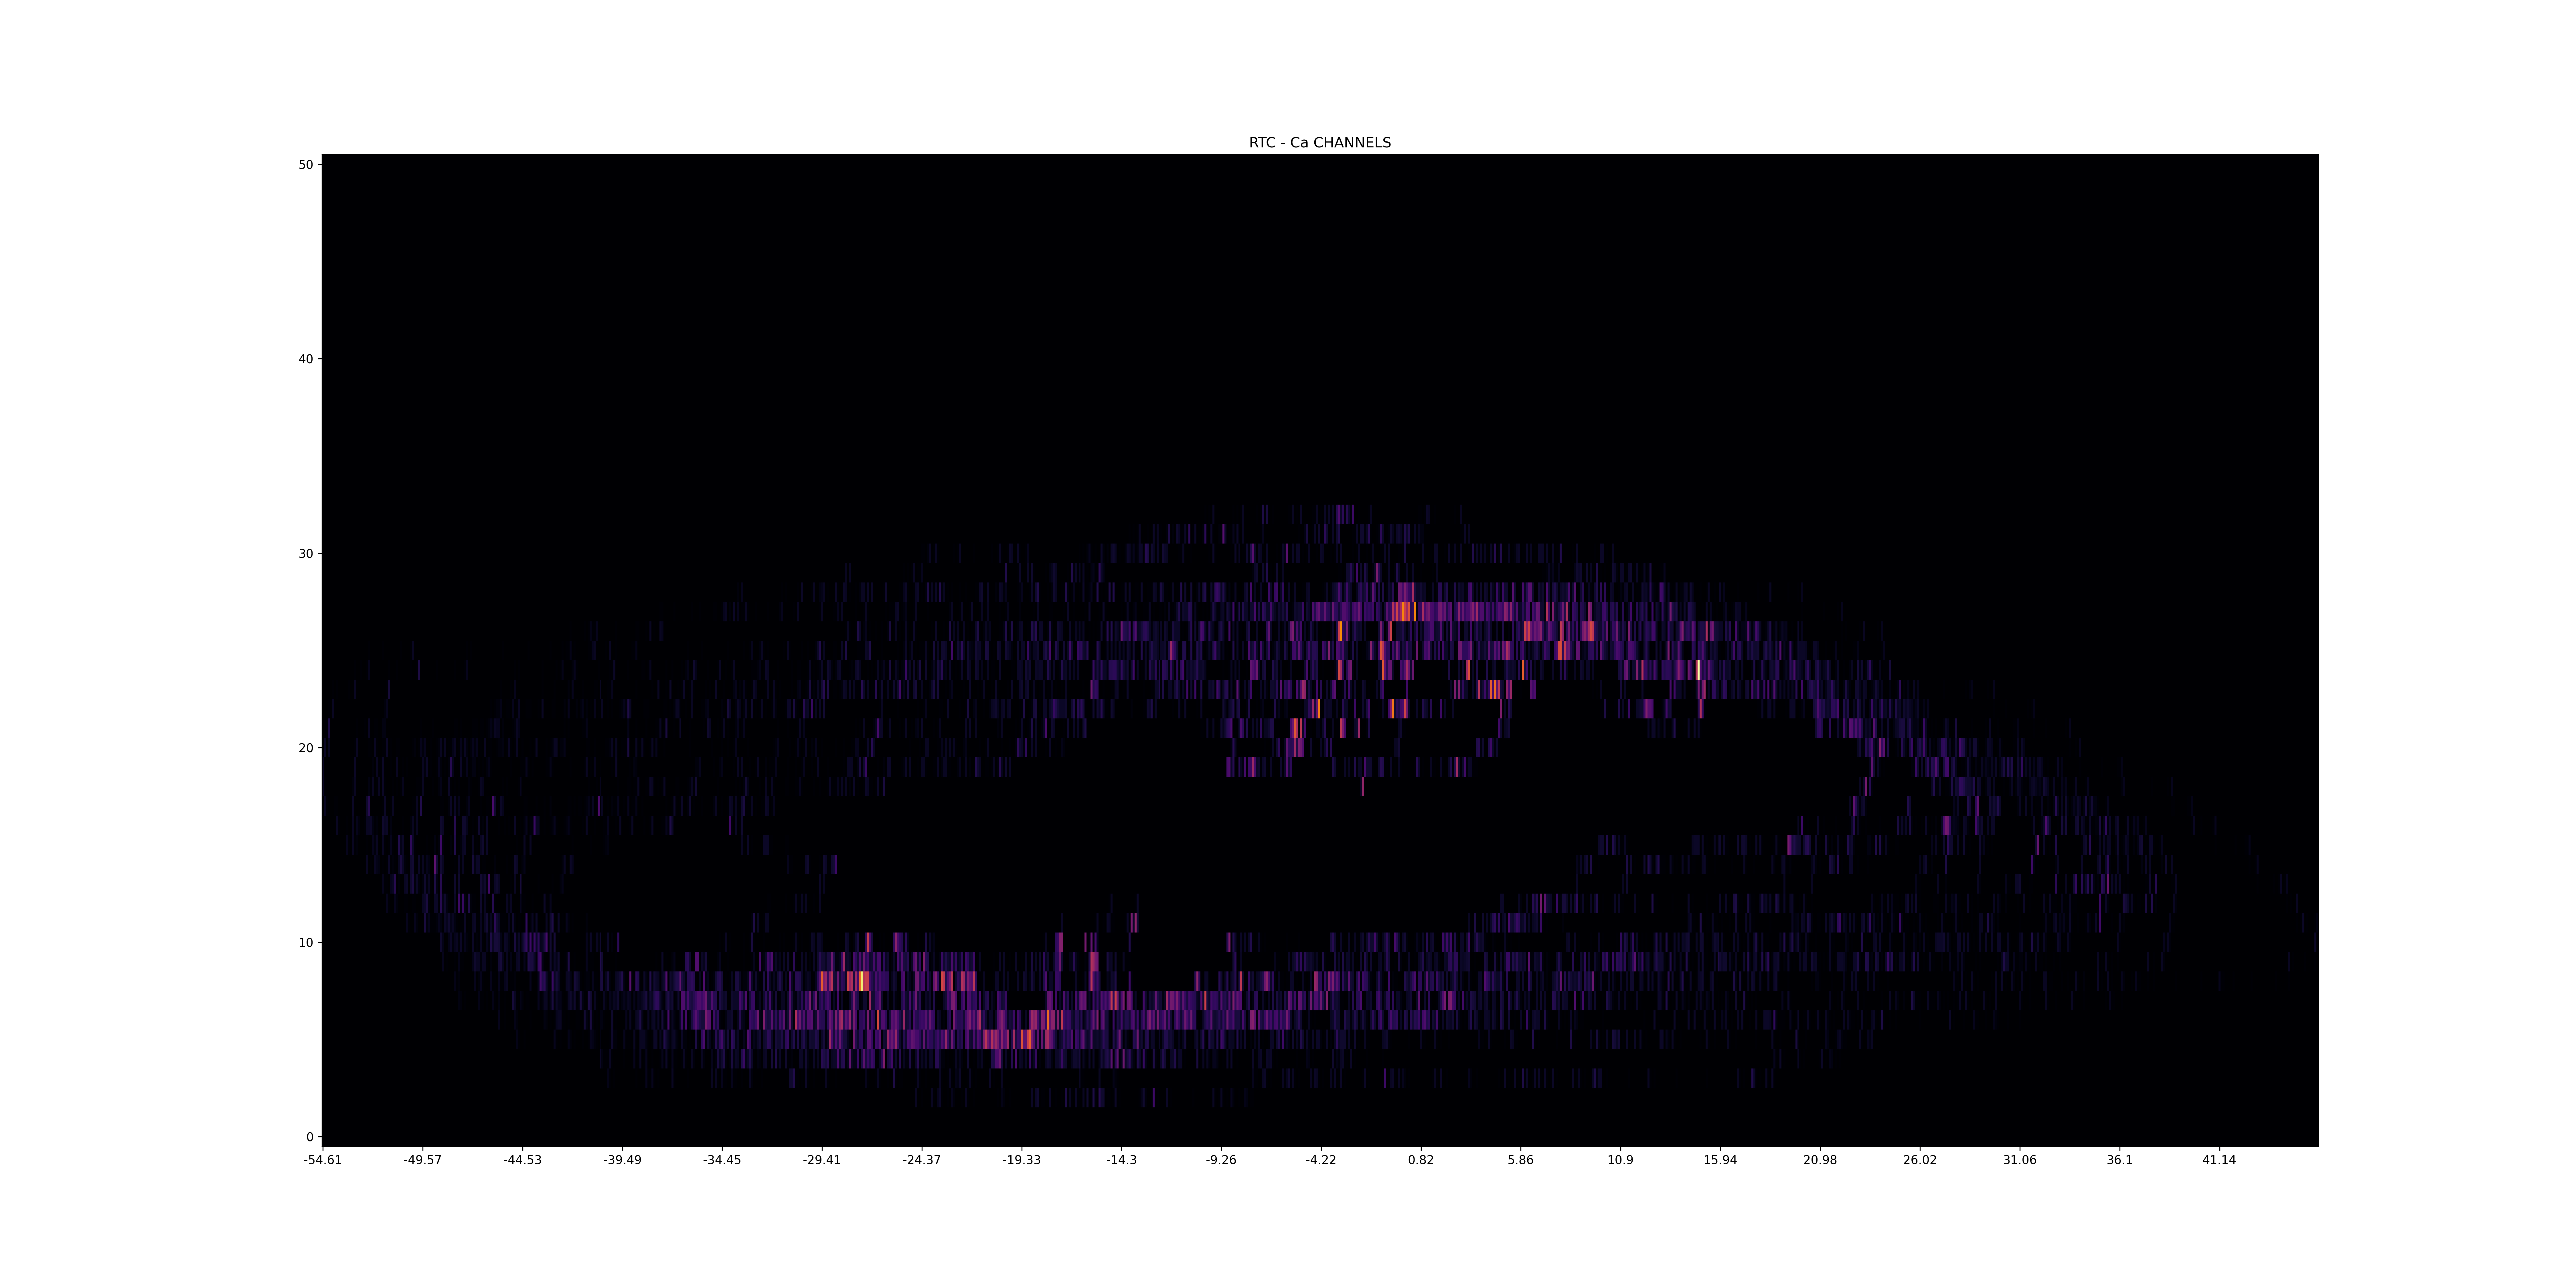
\includegraphics[width=.45\linewidth,valign=m]{Figures/50/Ca_RTC_.png} \\
    Gillespie &
    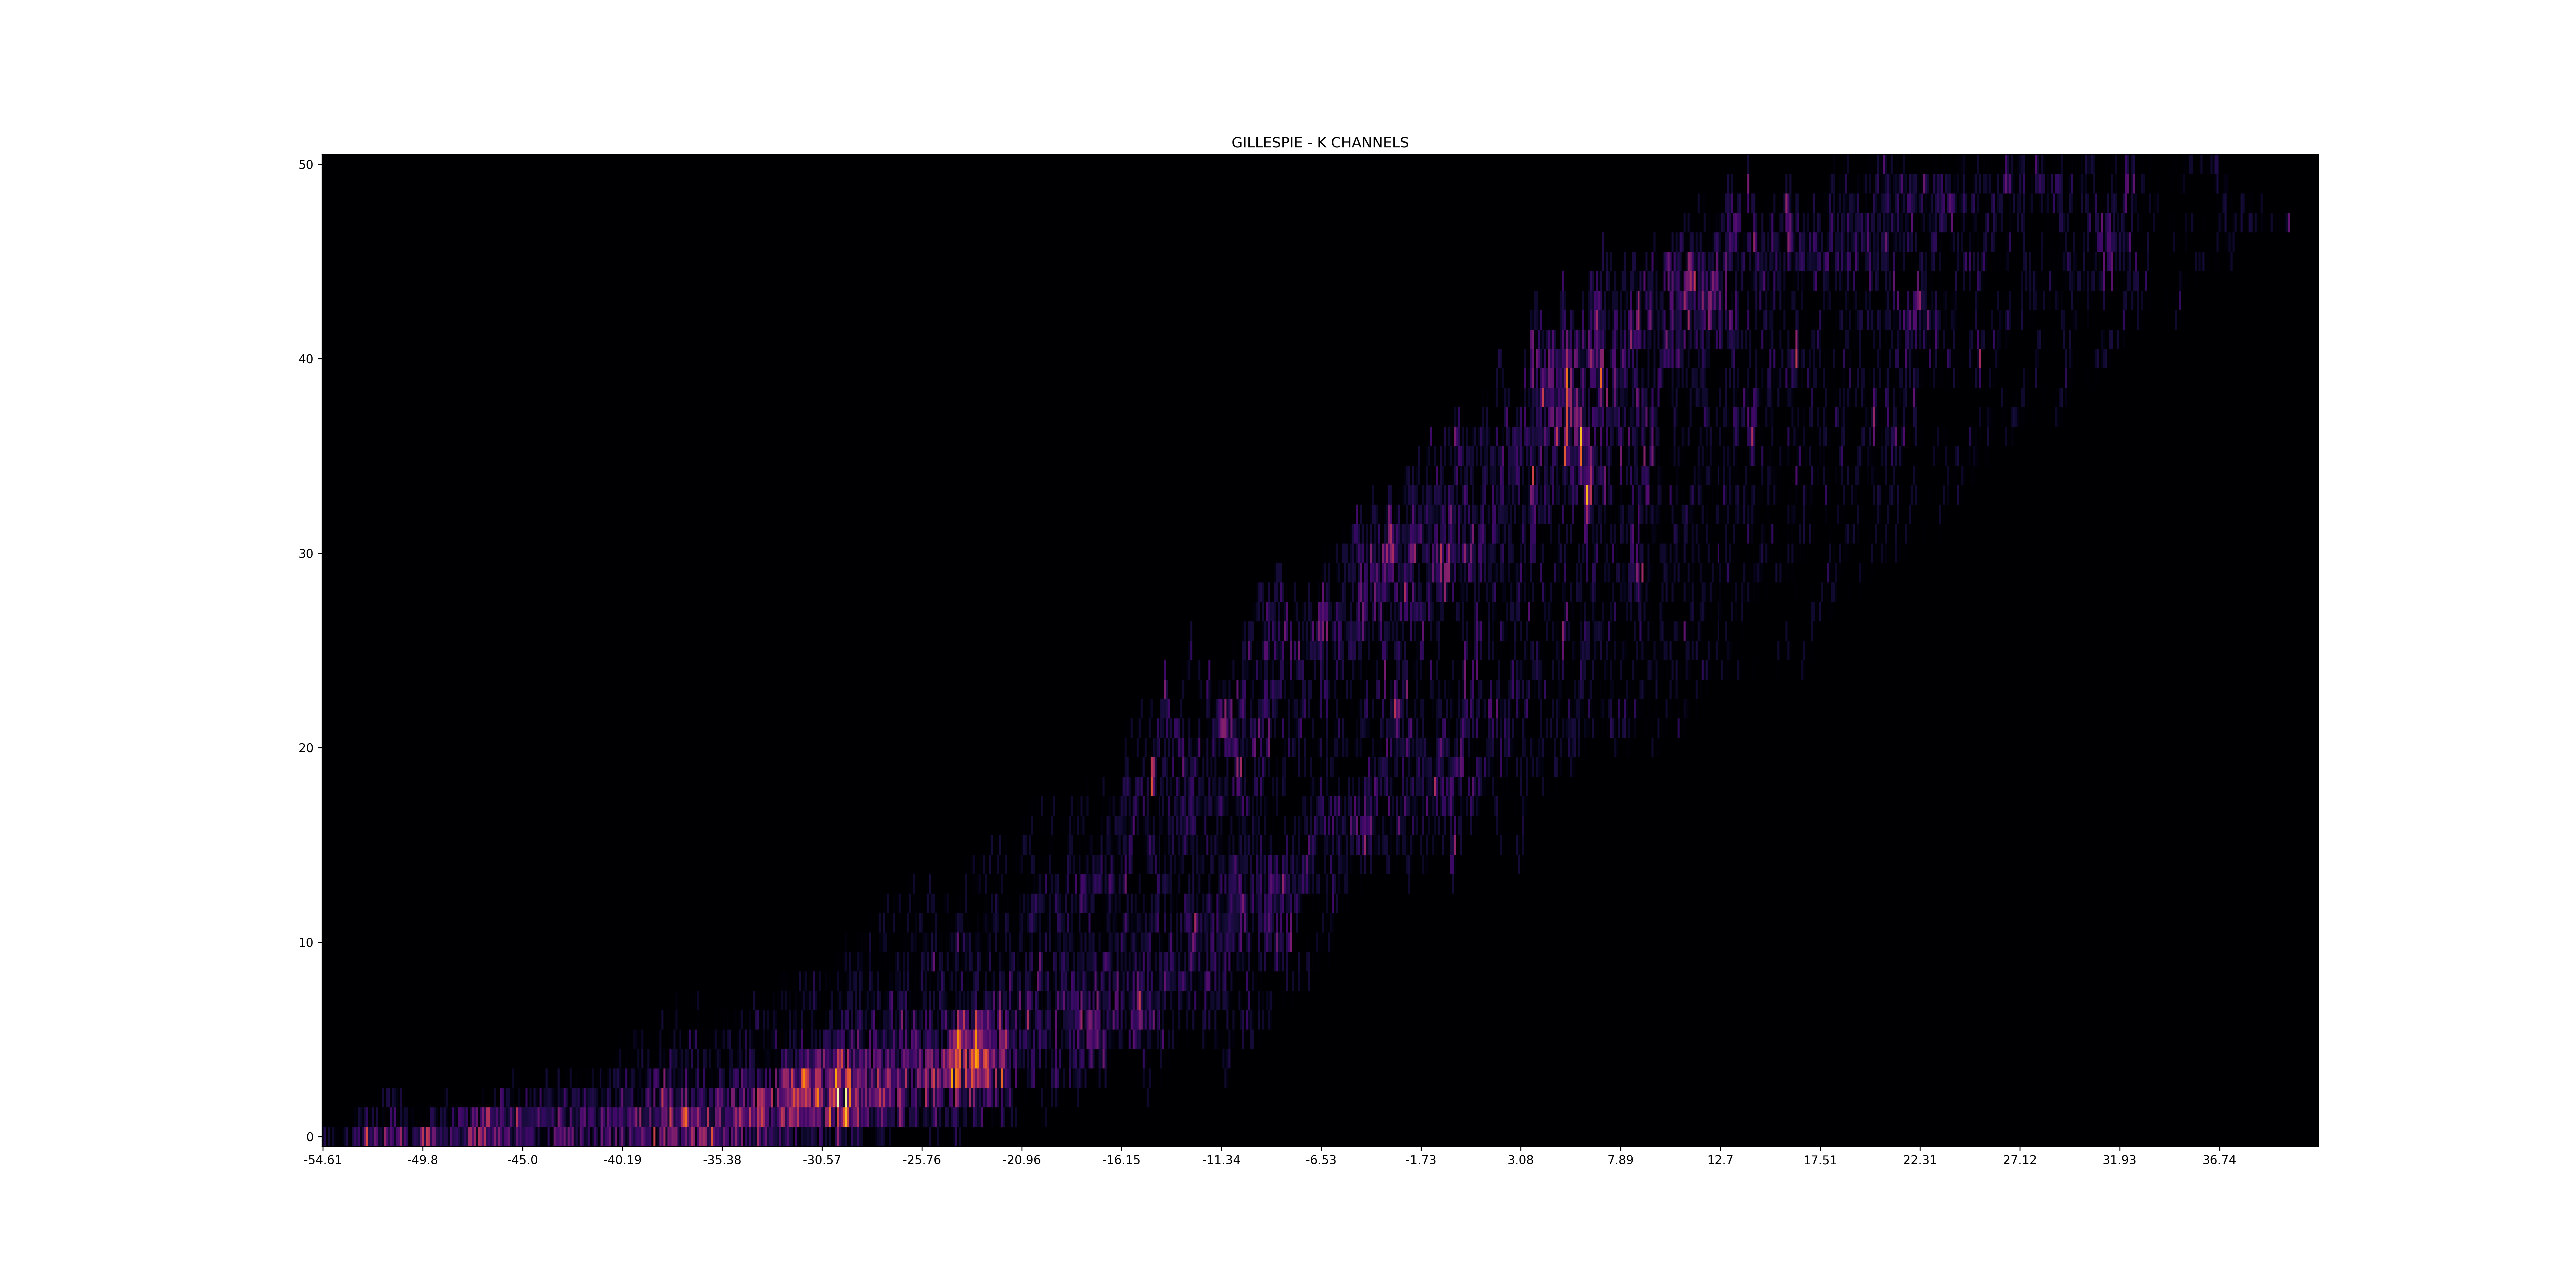
\includegraphics[width=.45\linewidth,valign=m]{Figures/50/K_GILLESPIE_.png} &
    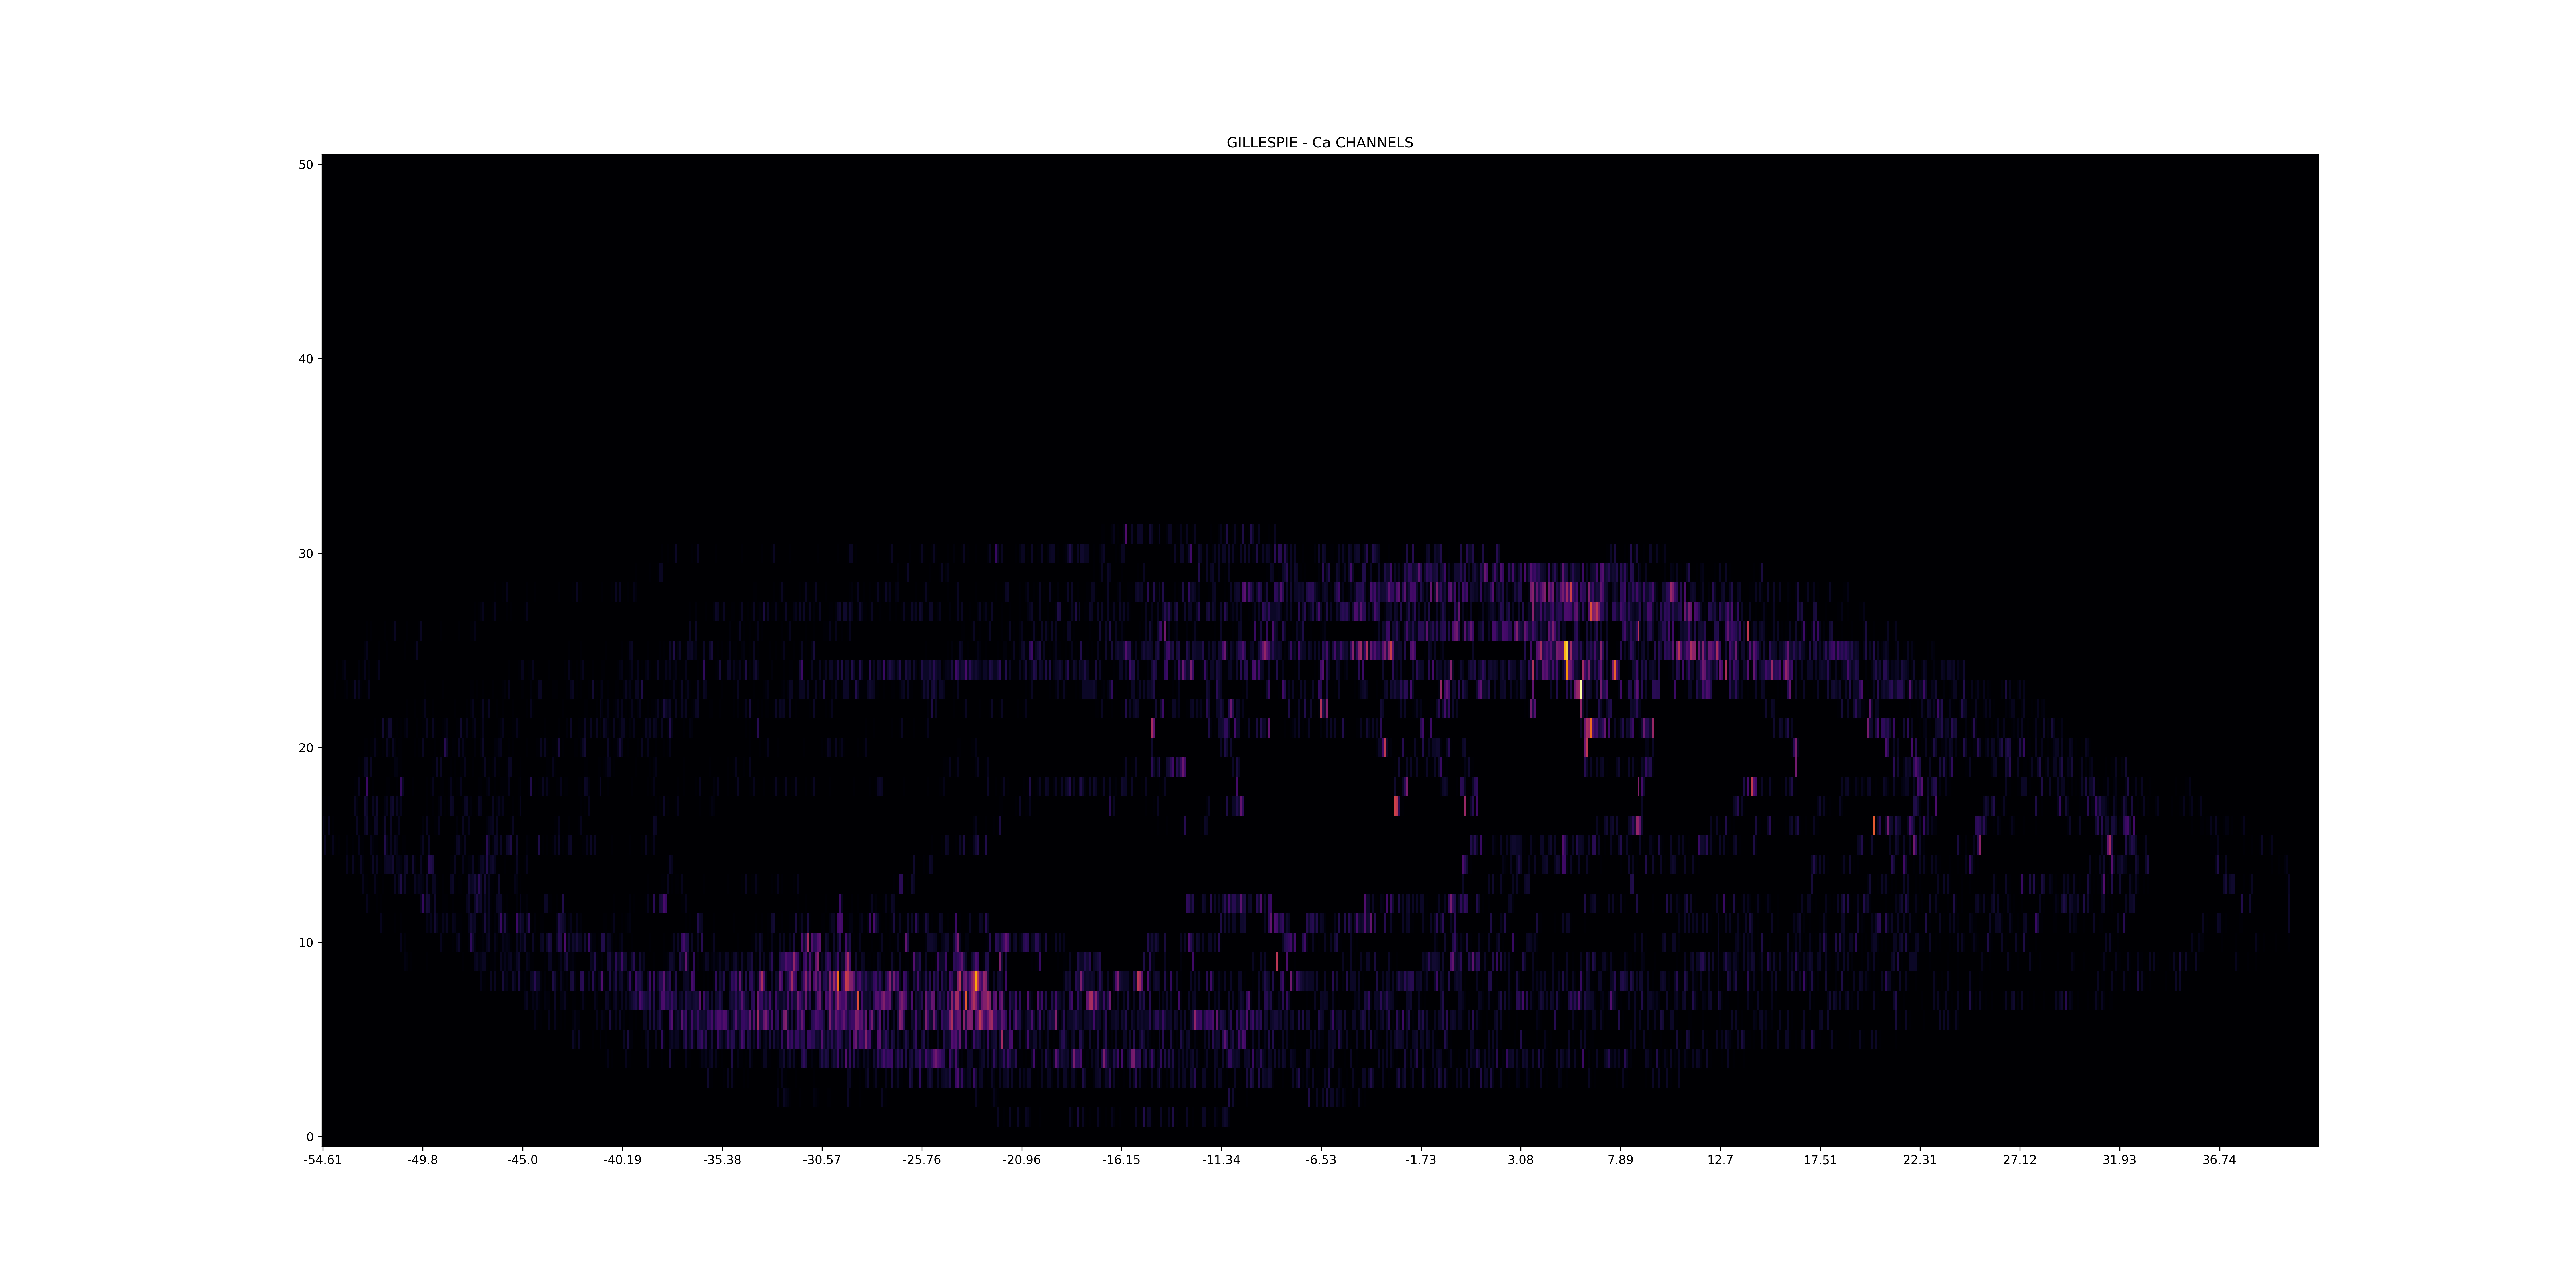
\includegraphics[width=.45\linewidth,valign=m]{Figures/50/Ca_GILLESPIE_.png} \\
    \end{tabular}
    \caption{Heatmap of the RTC and Gillespie representations using fifty channels for each type}
    \label{tab:my_label}
\end{table}

\begin{table}[]
    \centering
    \begin{tabular}{ccc}
    & Potassium & Calcium\\
    RTC &
    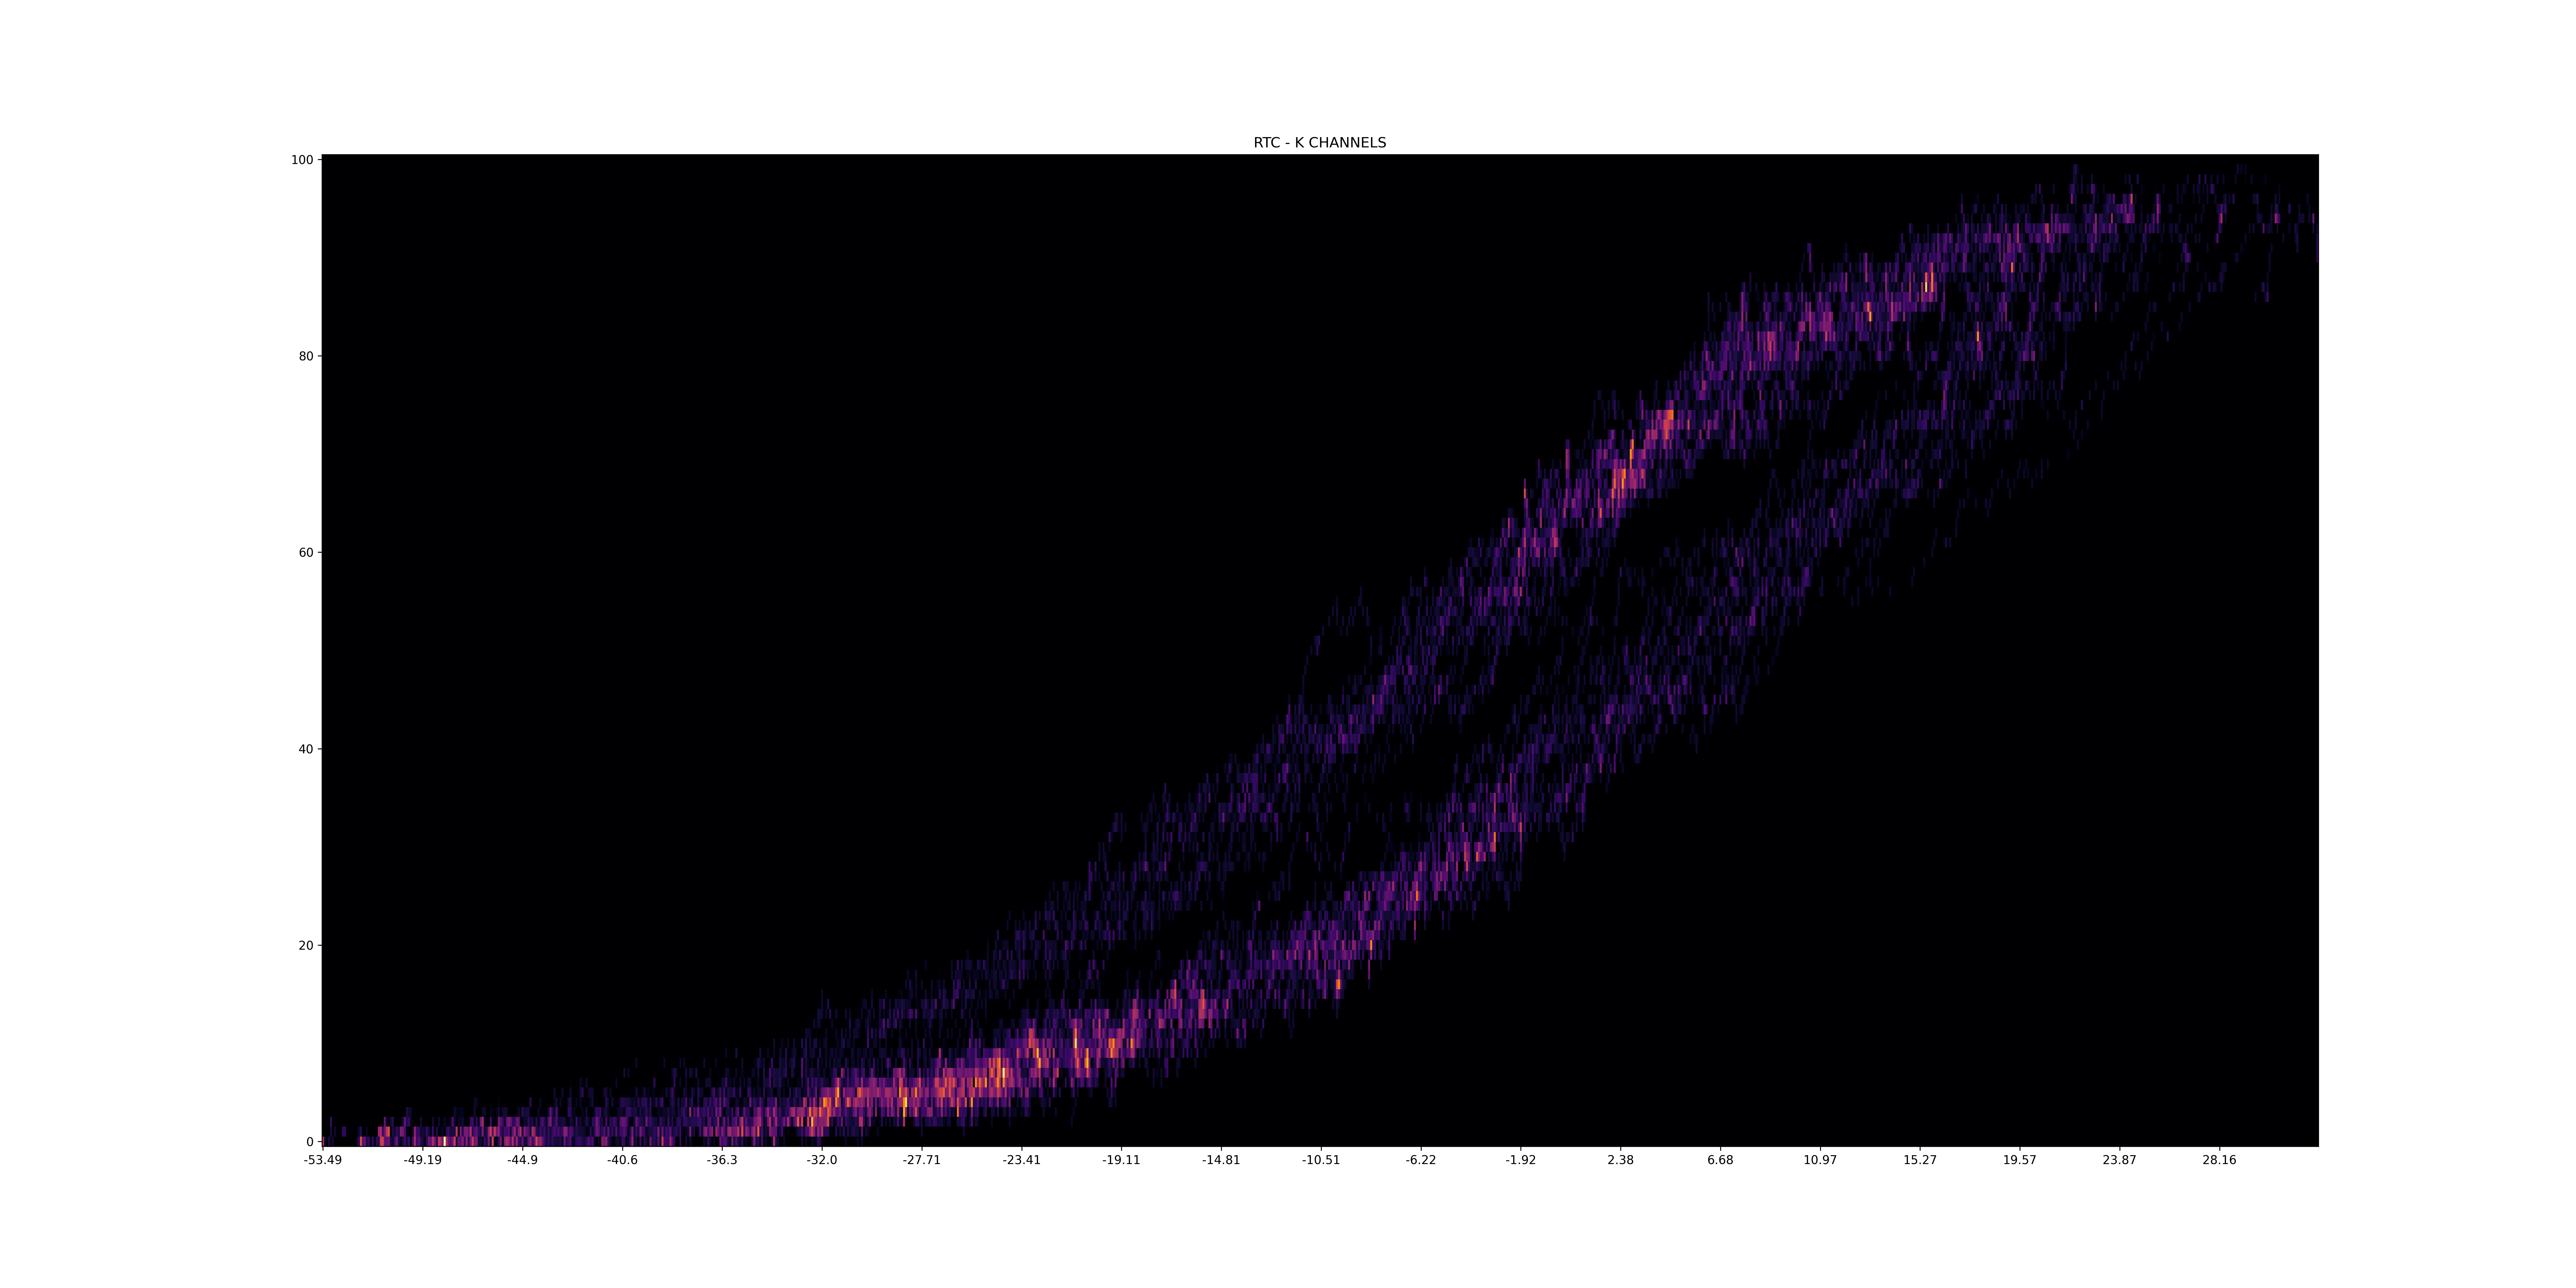
\includegraphics[width=.45\linewidth,valign=m]{Figures/100/K_RTC_.png} &
    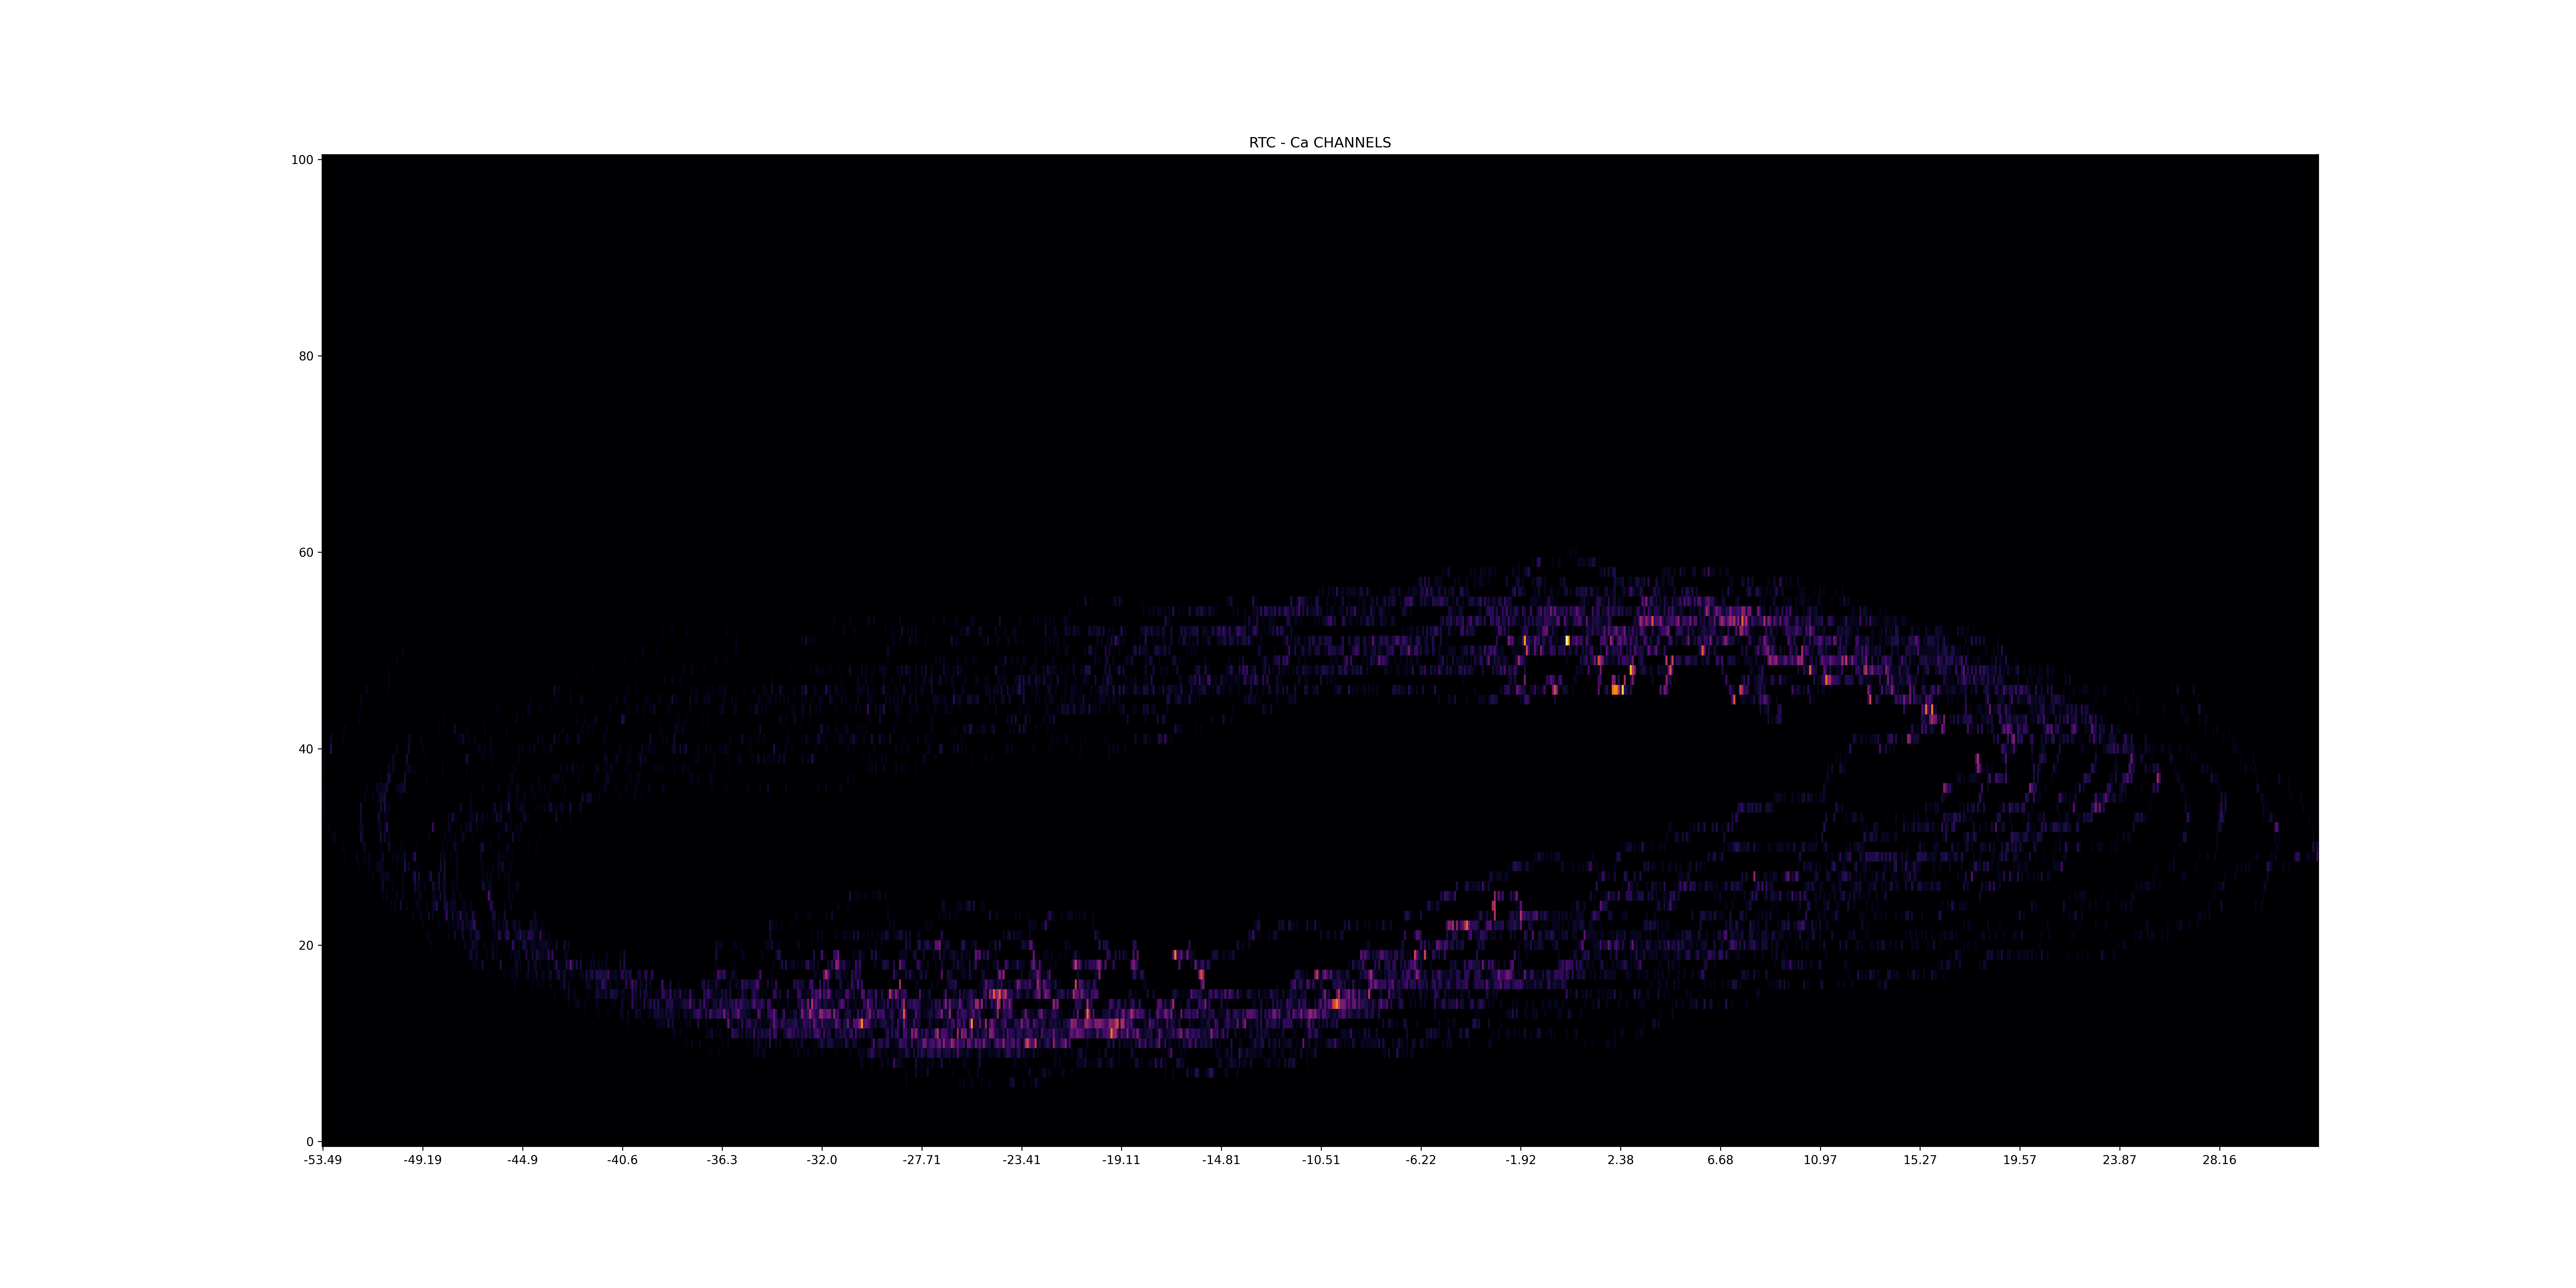
\includegraphics[width=.45\linewidth,valign=m]{Figures/100/Ca_RTC_.png} \\
    Gillespie &
    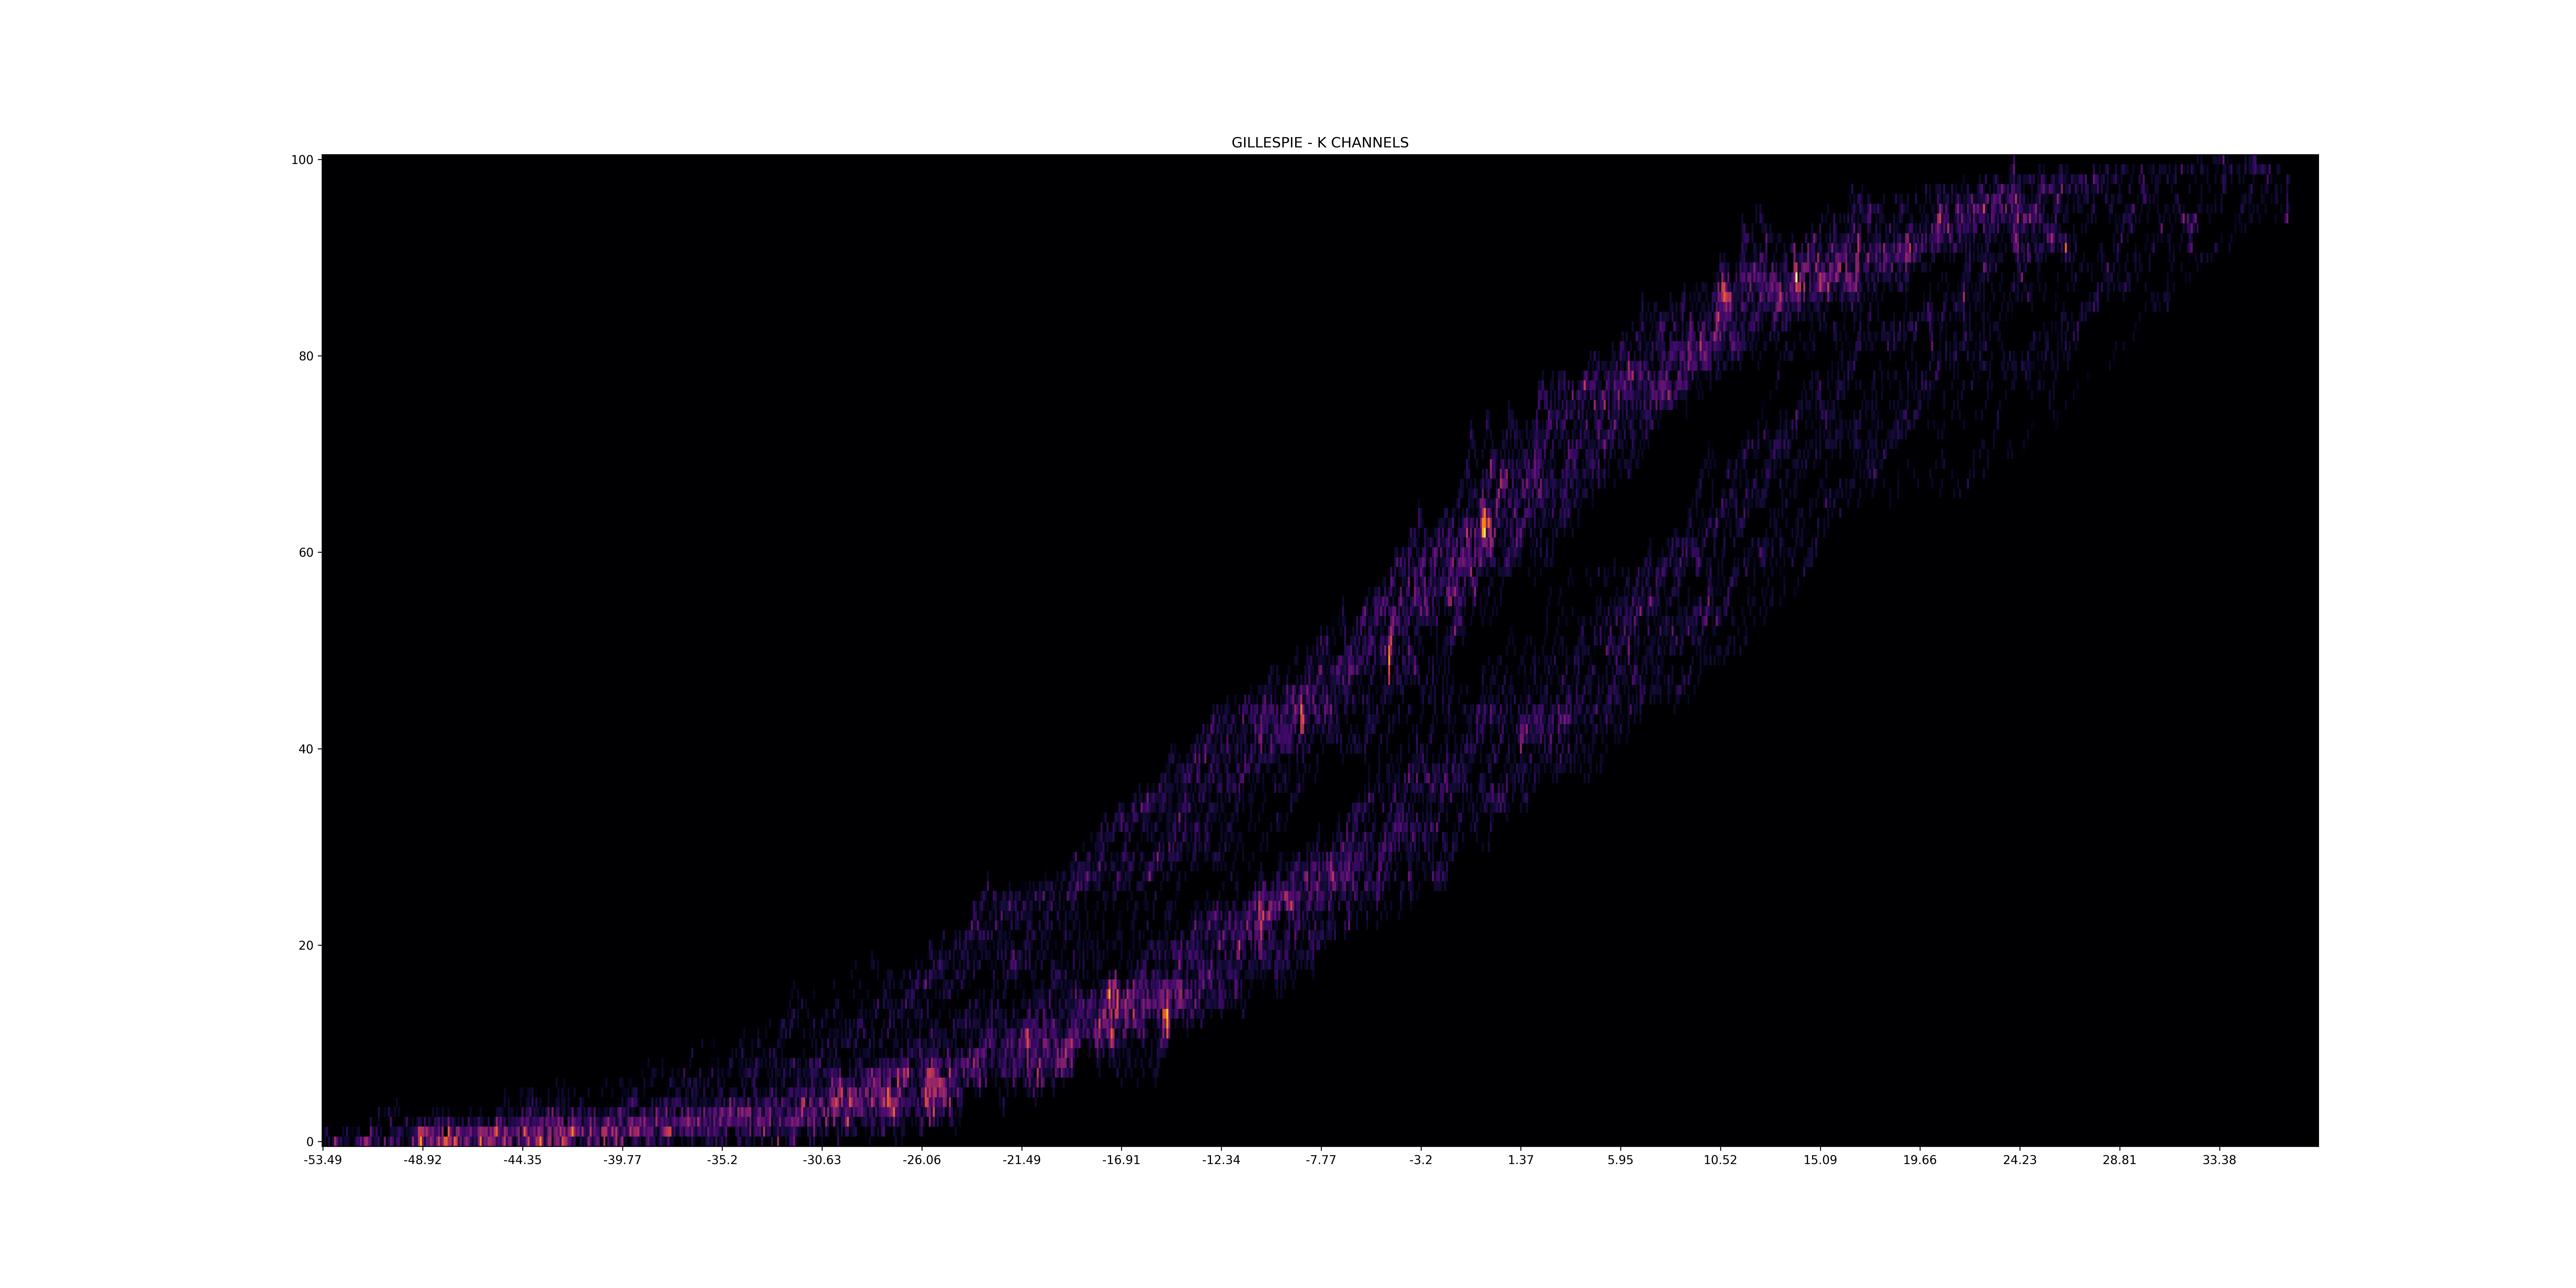
\includegraphics[width=.45\linewidth,valign=m]{Figures/100/K_GILLESPIE_.png} &
        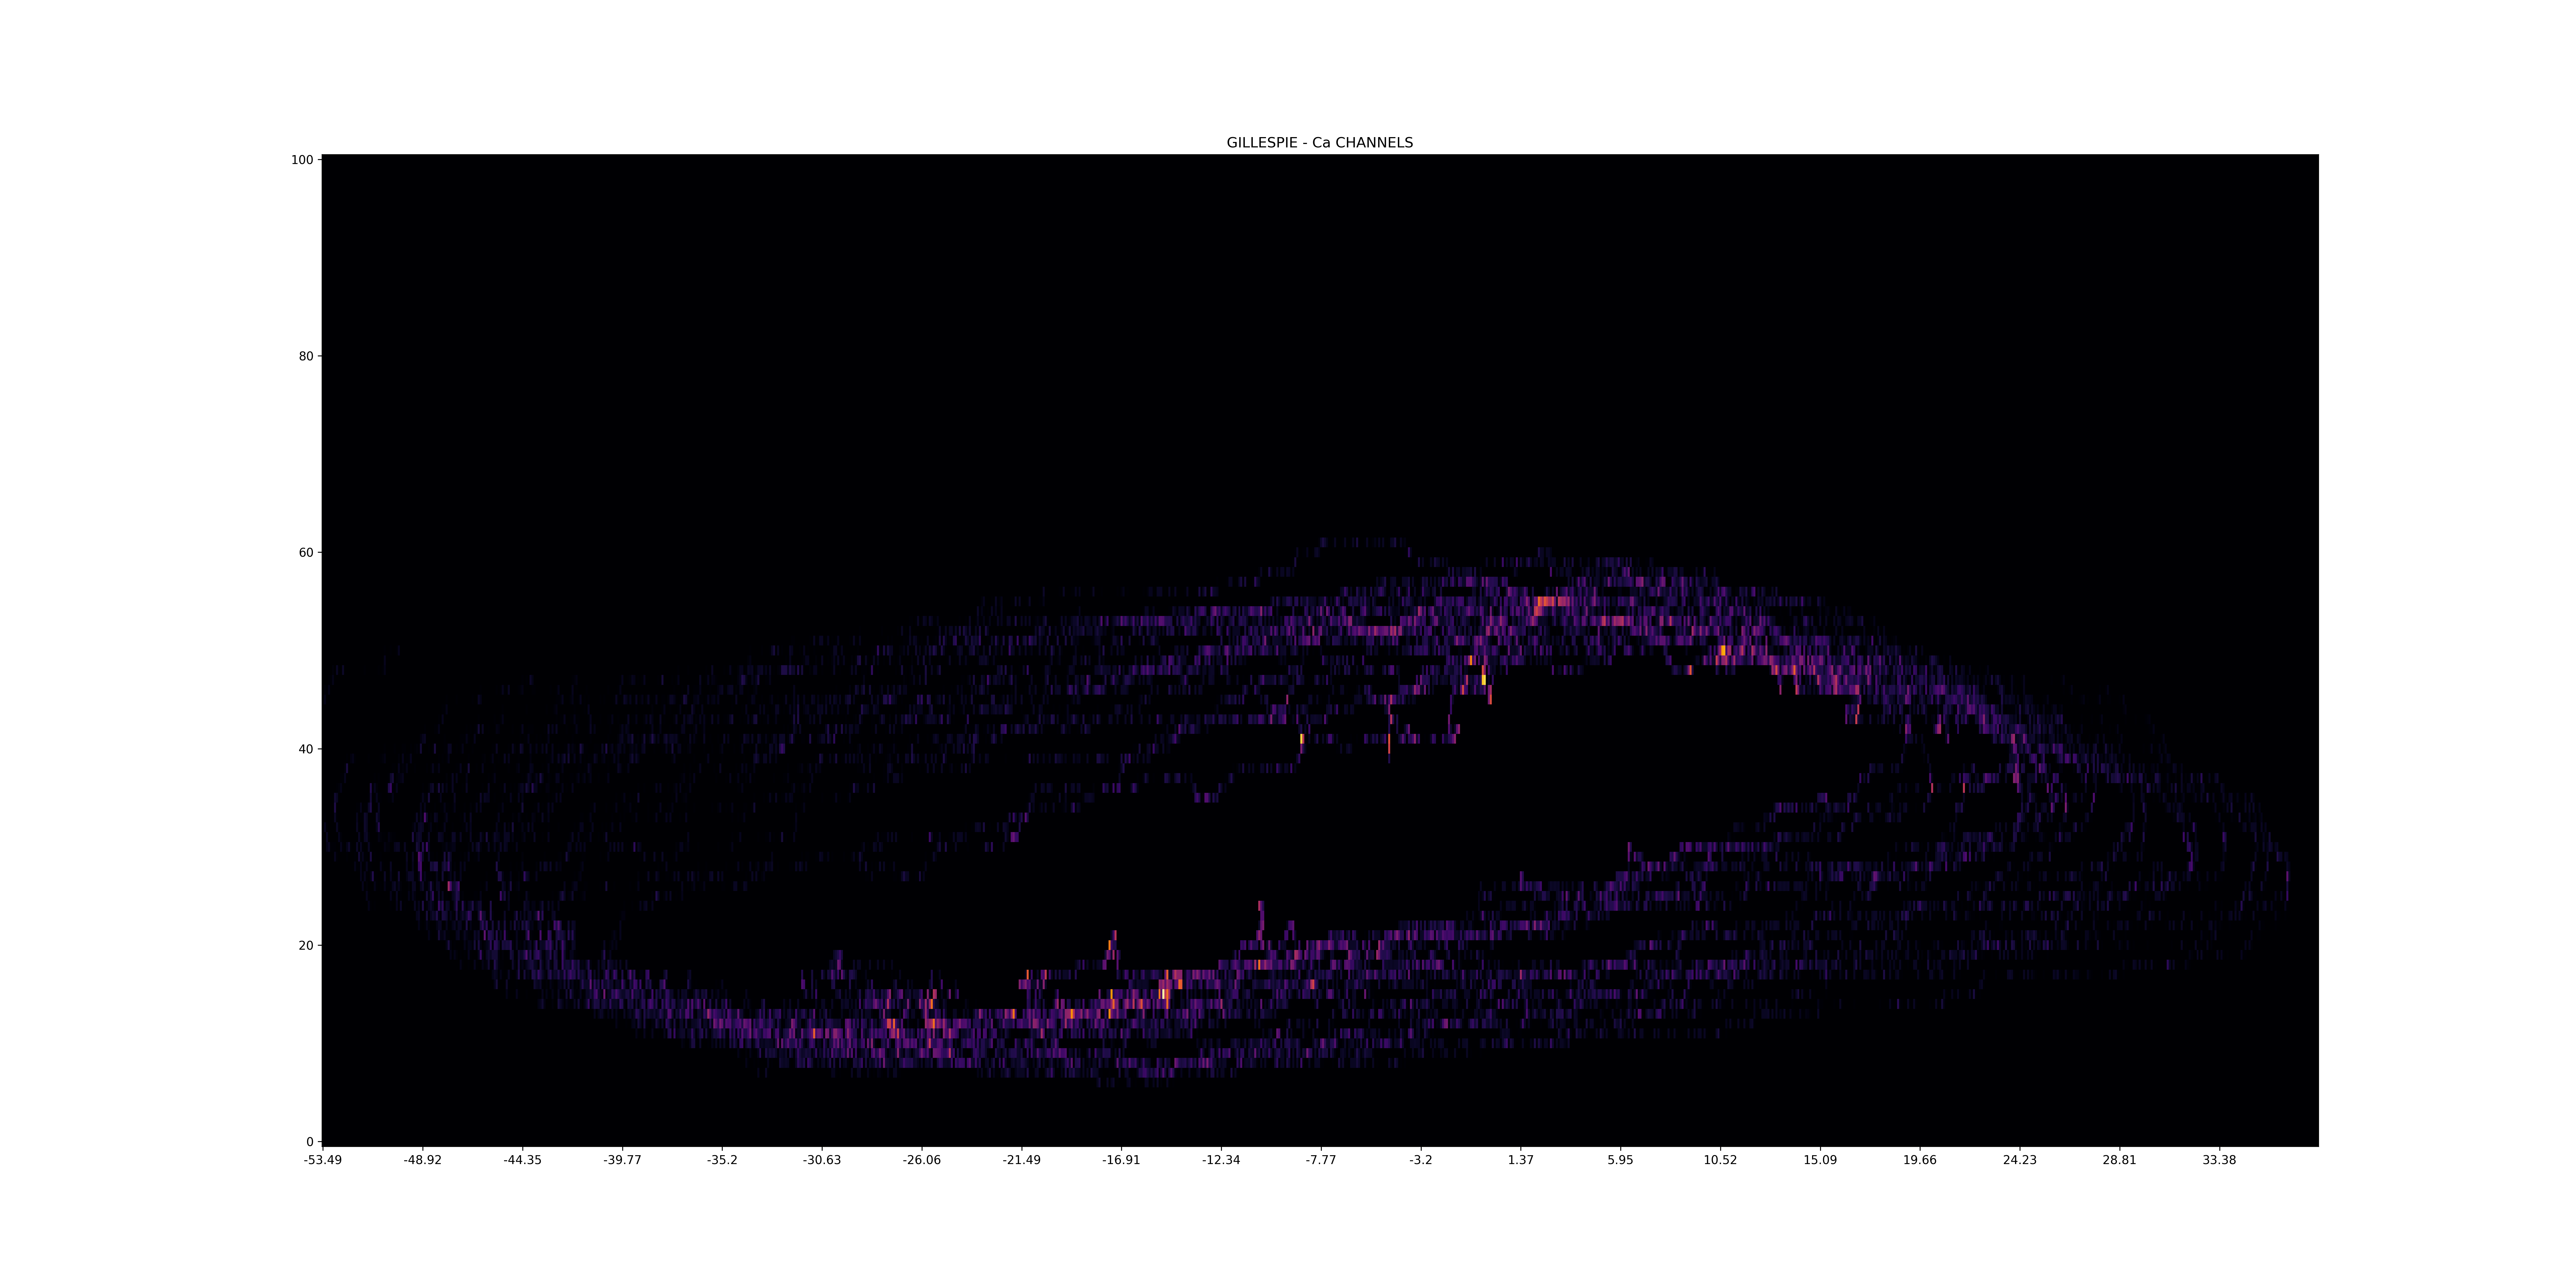
\includegraphics[width=.45\linewidth,valign=m]{Figures/100/Ca_GILLESPIE_.png} \\
    \end{tabular}
    \caption{Heatmap of the RTC and Gillespie representations using one hundred channels for each type}
    \label{tab:my_label}
\end{table}
